% !TeX program = xelatex
% Overleaf 使用说明：
% 1. 将本文件上传为 main.tex。
% 2. Overleaf 编译器选择 XeLaTeX。
% 3. 本文件已内置参考文献条目，不依赖 references.bib。
% 4. 本版重点更新实验设计、可落地数据处理管线、图结构/GNN 基线与量化贡献表。

\documentclass[UTF8,a4paper,10pt,twocolumn,fontset=fandol]{ctexart}

% ---------- 页面与字体 ----------
\usepackage[left=1.65cm,right=1.65cm,top=1.75cm,bottom=1.9cm,columnsep=0.72cm]{geometry}
\setlength{\parindent}{2em}
\setlength{\parskip}{0.15em}
\linespread{1.03}

% ---------- 常用宏包 ----------
\usepackage{amsmath,amssymb,amsfonts}
\usepackage{booktabs,tabularx,multirow,makecell,array}
\usepackage{graphicx}
\usepackage{subcaption}
\usepackage{float}
\usepackage{stfloats}
\usepackage{enumitem}
\usepackage{xcolor}
\usepackage{url}
\usepackage[hidelinks]{hyperref}
\usepackage[numbers,sort&compress]{natbib}
\usepackage[ruled,vlined,linesnumbered]{algorithm2e}
\usepackage{tikz}
\usetikzlibrary{arrows.meta,positioning,shapes.geometric}
\usepackage{balance}

% ---------- 表格列类型 ----------
\newcolumntype{Y}{>{\raggedright\arraybackslash}X}
\newcolumntype{C}[1]{>{\centering\arraybackslash}p{#1}}
\newcolumntype{L}[1]{>{\raggedright\arraybackslash}p{#1}}
\renewcommand{\arraystretch}{1.12}
\setlength{\tabcolsep}{4pt}

% ---------- 列表压缩 ----------
\setlist[itemize]{leftmargin=1.3em,itemsep=0.1em,topsep=0.2em}
\setlist[enumerate]{leftmargin=1.5em,itemsep=0.1em,topsep=0.2em}
\setlist[description]{leftmargin=0em,labelindent=0em,itemsep=0.1em,topsep=0.2em}

% ---------- 常用命令 ----------
\newcommand{\isic}{ISIC 2024 SLICE-3D Permissive}
\newcommand{\pad}{PAD-UFES-20}
\newcommand{\modelname}{LGKE-GNN}

% ---------- 标题信息 ----------
\title{\vspace{-1.2em}\textbf{多模态皮肤病变风险筛查与公平性评估：\\面向 ISIC 2024 SLICE-3D 的可复现实验设计}}
\author{\small
2354100 郝哲逸 \quad
2353594 姜政言 \quad
2354356 林青滢 \quad
2353833 高文昊
}
\date{\small 最终研究报告}

\begin{document}
\maketitle
\vspace{-1.2em}

\begin{abstract}
本文研究图像与临床元数据融合条件下的皮肤病变风险筛查。针对 ISIC 2024 SLICE-3D 中同一患者多病灶、元数据丰富且类别极端不均衡的特点，本文提出 \modelname{}，一种受知识图谱自编码思想启发的异构图多模态模型。该模型将病灶样本、患者上下文、解剖部位、年龄段、尺寸分箱、视觉近邻和知识原型统一到 fold-specific 病灶图中，并通过关系特异 GraphSAGE 聚合与知识原型注意力学习联合风险表示。实验采用严格的患者级五折交叉验证，并以 pAUC@TPR$\geq0.80$、AUPRC、AUROC、FNR、Brier score、ECE 和子群差异作为主要评价维度。在内部患者级测试中，\modelname{} 达到 $77.94\pm7.48$ 的 pAUC 和 $94.15\pm1.60$ 的 AUROC，优于表格、图像和常规多模态融合基线；AUPRC 为 $7.08\pm3.97$，接近最强门控融合基线。PAD-UFES-20 外部验证进一步表明，零样本跨域迁移存在显著性能下降，而 PAD-only fine-tune 能明显恢复目标域判别性能。结果说明，显式建模患者--病灶--属性--视觉近邻关系能够提升 3D-TBP 筛查场景中的高灵敏度风险排序，但跨设备域迁移和子群稳定性仍是后续研究的关键问题。

\textbf{关键词：} 多模态学习；皮肤病变；ISIC 2024；图神经网络；数据融合；公平性评估
\end{abstract}

\section{引言}

皮肤病变风险筛查是医学图像分析中最具有临床转化潜力、同时也最容易受到数据分布和评价协议影响的任务之一。早期深度学习研究已经证明，端到端卷积神经网络能够在受控图像分类任务中达到接近皮肤科医生的诊断水平 \cite{esteva2017dermatologist}；随后，HAM10000、ISIC 系列数据集和相关挑战进一步推动了皮肤病变分类从小规模实验走向标准化基准评估 \cite{tschandl2018ham10000,cassidy2022isic}。然而，真实筛查场景与传统“单张皮肤镜图像二分类”设定存在显著差异：一方面，恶性样本通常远少于良性样本，模型需要在极高灵敏度区域仍保持可用的特异度；另一方面，临床判断并不只依赖单个病灶的局部视觉形态，而会同时参考患者年龄、性别、解剖部位、病灶尺寸以及同一患者其他病灶的相对异常性 \cite{rotemberg2021patient}。因此，皮肤病变 AI 的核心挑战已经从“能否识别一张图像中的病灶”转变为“如何在类别极端不均衡、患者上下文丰富、跨设备域迁移明显且存在公平性风险的条件下，进行可信的风险排序”。

ISIC 2024 SLICE-3D 为这一问题提供了新的研究场景。与以往主要基于皮肤镜图像的数据集不同，SLICE-3D 来源于三维全身摄影（3D Total Body Photography, 3D-TBP）中提取的病灶裁剪图像，数据描述论文报告其包含约 40 万个 3D-TBP 病灶裁剪样本，目标是支持从全身摄影场景中进行皮肤癌检测 \cite{kurtansky2024slice3d}。ISIC 2024 挑战进一步将评价重点放在高灵敏度区间，采用 TPR 高于 80\% 区间的 partial AUC 作为主要指标 \cite{isic2024challenge}。这一评价方式与筛查任务高度一致：在临床筛查中，漏诊恶性病灶的代价通常高于增加一定数量的假阳性，但如果模型只追求召回而产生过多假阳性，也会增加后续随访、活检和医疗资源负担。因此，单独报告 AUROC 或 accuracy 不足以支撑结论，本文同时报告 pAUC、AUPRC、固定高灵敏度阈值下的 FNR、校准误差以及子群差异。

本文的研究动机来自 SLICE-3D 数据结构本身。3D-TBP 采集不是孤立图像采集，而是一次扫描中记录同一患者的多个病灶、病灶位置及相关临床元数据；这种 patient-level contextual information 与皮肤科医生常用的 ``ugly duckling'' 判断逻辑一致，即通过比较同一患者内部多个病灶的相似性和异常性来辅助识别高风险病灶 \cite{rotemberg2021patient,kurtansky2024slice3d}。然而，许多常规图像模型或图像--元数据融合模型仍将每个病灶作为相互独立的样本，只在特征层拼接图像 embedding 与表格变量。这种处理方式忽略了患者、病灶、解剖部位、年龄段、尺寸分箱和视觉近邻之间天然存在的关系结构，也难以解释模型性能提升究竟来自视觉特征、临床元数据还是患者上下文。

为此，本文提出一个面向 ISIC 2024 SLICE-3D 的可复现多模态风险筛查框架。该框架从原始图像、元数据和标签构建统一 manifest、患者级划分、fold-specific 预处理器和异构病灶图，并在同一评估协议下比较表格模型、CNN、视觉 Transformer、冻结医学图像--文本基础模型特征、常规门控融合模型和图结构多模态模型。核心方法 LGKE-GNN 受知识图谱自编码思想启发，将病灶样本、患者上下文、属性节点和视觉近邻组织为异构图，并利用关系特异 GraphSAGE 聚合和知识原型注意力学习图像、元数据和图结构的联合表示 \cite{hamilton2017graphsage,liu2021kgae}。与传统 late fusion 不同，LGKE-GNN 不仅融合单个样本的多模态特征，还显式建模“同患者病灶”“同解剖部位/属性”“视觉相似病灶”之间的关系。

本文的主要贡献包括四点。第一，围绕 SLICE-3D 构建严格的患者级可复现实验协议，避免同一患者病灶跨训练集和测试集造成信息泄漏，并保证缺失值填补、标准化、类别词表、分箱边界和图边构建均只在训练折上拟合 \cite{cassidy2022isic,rotemberg2021patient}。第二，在常规图像模型、表格模型和多模态融合模型之外，引入 LGKE-GNN，将 3D-TBP 场景中的患者上下文和视觉相似性转化为可学习的异构图结构。第三，采用与 ISIC 2024 挑战一致的高灵敏度 pAUC 作为主指标，同时报告 AUPRC、AUROC、FNR、Brier score、ECE 和推理成本，以避免在极端类别不均衡任务中只依赖单一总体指标 \cite{isic2024challenge}。第四，使用 PAD-UFES-20 作为外部验证和 Fitzpatrick 皮肤类型公平性补充数据源，评估模型在智能手机临床图像域上的迁移能力和子群稳定性 \cite{pacheco2020padufes,daneshjou2022disparities,groh2021fitzpatrick17k}。通过上述设计，本文试图回答一个更具体的问题：在 3D-TBP 皮肤病变筛查中，显式建模患者--病灶--属性--视觉近邻关系，是否能够比单纯图像分类或简单多模态拼接更有效地支持高灵敏度风险筛查？

\section{相关工作}

\subsection{皮肤病变图像分类与公开基准}

皮肤病变自动分类最早主要围绕皮肤镜图像展开，典型路线是使用卷积神经网络从图像像素中学习恶性/良性或多类别诊断表示。Esteva 等人证明，大规模 CNN 在若干皮肤癌分类任务中能够达到接近皮肤科医生的表现，这一工作奠定了深度学习用于皮肤病变识别的基础 \cite{esteva2017dermatologist}。随后，HAM10000 提供了 10,015 张多来源皮肤镜图像，缓解了早期皮肤病变数据规模小、类别覆盖不足的问题 \cite{tschandl2018ham10000}。ISIC 系列挑战进一步推动了统一训练/测试划分、公开排行榜和标准化指标的发展，但 Cassidy 等人也指出，ISIC 数据集中存在重复样本、数据来源偏差和评价协议不一致等问题，若不进行患者级划分和去泄漏处理，模型性能可能被高估 \cite{cassidy2022isic}。

近年来，研究重点逐渐从单病灶皮肤镜图像扩展到患者级临床上下文。Rotemberg 等人构建的 SIIM-ISIC 2020 数据集明确引入 patient id，使同一患者的多个病灶能够被关联起来，并指出真实临床判断通常依赖患者级多病灶上下文，而不是孤立地观察一张图像 \cite{rotemberg2021patient}。ISIC 2024 SLICE-3D 则进一步将任务推进到 3D-TBP 场景：模型面对的是从全身摄影中裁剪出的非皮肤镜病灶图像，同时伴随患者、解剖部位、尺寸和 TBP Visualizer 等结构化元数据 \cite{kurtansky2024slice3d}。与传统 dermoscopy benchmark 相比，SLICE-3D 更接近大规模筛查和远程医疗应用，也要求模型处理更强的类别不均衡、更复杂的患者内相关性和更明显的采集域差异。本文的实验设计继承 ISIC benchmark 的标准化思想，但进一步强调患者级划分、训练折内预处理、外部验证和高灵敏度区间指标 \cite{cassidy2022isic,isic2024challenge}。

\subsection{图像--元数据多模态融合}

皮肤病变诊断天然是多模态问题。除图像外，年龄、性别、解剖部位、病灶尺寸、病史和皮肤类型等信息都会影响临床风险判断。早期多模态皮肤病变分类工作已尝试将临床图像、皮肤镜图像和患者元数据联合输入深度模型，以提升相较单模态图像分类的表现 \cite{yap2018multimodal}。Wang 等人提出的 adversarial multimodal fusion with attention mechanism 进一步说明，不同视觉模态之间既存在互补信息，也存在可通过注意力和对抗训练约束的相关信息 \cite{wang2022amfam}。近期基于 ISIC 派生数据的研究也系统比较了 dermoscopic images 与 clinical metadata 的融合效果，表明元数据在部分设置下能够改善分类性能，但其贡献依赖于划分协议、类别分布和融合结构 \cite{ahammed2025metadata}。

除传统 CNN/MLP 融合外，医学图像--文本基础模型也为皮肤病变分析提供了新的特征来源。MONET 通过医学文献中的图像--文本信息学习医学概念相关表示，可用于提取更具语义性的冻结视觉特征或概念提示特征 \cite{kim2024monet}。这类模型的优势在于能够将视觉模式与医学概念空间对齐，从而提高可解释性和跨任务迁移能力；但在 SLICE-3D 场景中，仅使用冻结 embedding 或文本提示仍无法直接建模同一患者内部的多病灶关系。因此，现有多模态方法虽然证明了图像和临床元数据融合的必要性，但多数方法仍停留在样本级特征拼接、门控或 cross-attention，尚未充分利用 3D-TBP 数据中天然存在的患者--病灶图结构。

\subsection{患者上下文建模与图神经网络}

患者上下文建模是本文与常规多模态融合的主要区别。对于同一患者，多个病灶之间并非独立同分布：某个病灶是否异常，往往取决于它相对于患者其他病灶的颜色、形状和尺寸差异 \cite{rotemberg2021patient}。这种关系可以自然表示为图：病灶是节点，同患者关系、解剖部位关系、元数据相似性和视觉近邻关系是边。图神经网络为这种结构化建模提供了基础工具。GraphSAGE 通过采样和聚合邻域特征实现 inductive node representation learning，适合处理训练时和测试时节点集合不同的场景 \cite{hamilton2017graphsage}；GAT 使用注意力权重区分不同邻居的重要性 \cite{velickovic2018gat}；GATv2 则改进了原始 GAT 的静态注意力限制，使邻居排序能够更依赖于查询节点本身 \cite{brody2022gatv2}。这些特性都适合用于病灶图中的关系聚合和测试样本接入。

医学知识图谱和图编码器也为本文的模型设计提供了启发。KGAE 将知识图谱视为视觉与文本之间的共享潜空间，通过知识驱动编码器和解码器完成医学报告生成 \cite{liu2021kgae}。本文不处理报告生成任务，也不使用文本重构损失，而是借鉴“图作为共享知识空间”的思想，将病灶、属性、患者上下文和视觉近邻组织为监督式风险筛查图。LGKE-GNN 中的知识原型注意力可被理解为一种面向皮肤病变筛查的轻量知识读取机制：模型既从局部邻域聚合患者内和视觉相似信息，也从训练折中学习到的属性组合、视觉聚类和元数据聚类原型中读取全局模式。相较于仅将 metadata 与 image embedding 拼接的 late fusion，这种设计更适合回答“图结构是否带来额外收益”这一研究问题。

\subsection{外部验证、公平性与可信评价}

皮肤病变 AI 的另一个关键问题是跨域泛化和公平性。PAD-UFES-20 由智能手机临床图像和患者临床特征组成，包含患者年龄、病灶位置、Fitzpatrick 皮肤类型和病灶直径等信息，与 ISIC 2024 的 3D-TBP 裁剪图像在采集设备、图像风格和诊断分布上均存在差异 \cite{pacheco2020padufes}。因此，将 PAD-UFES-20 作为外部验证集可以检验模型是否只是拟合 SLICE-3D 内部分布，还是能够在更接近移动端临床采集的场景中保持稳定风险排序。与此同时，PAD-UFES-20 中的 Fitzpatrick 字段也为皮肤类型子群分析提供了补充信息 \cite{pacheco2020padufes}。

公平性研究表明，皮肤科 AI 在不同肤色、疾病类型和数据来源上的性能可能存在显著差异。Daneshjou 等人基于 Diverse Dermatology Images 数据集发现，现有 dermatology AI 模型在深色皮肤和少见疾病上的表现存在明显局限 \cite{daneshjou2022disparities}；Groh 等人构建 Fitzpatrick 17k 数据集并指出，深色皮肤样本在公开数据中往往不足，模型在接近训练分布的肤色类型上表现更好 \cite{groh2021fitzpatrick17k}。这些工作说明，皮肤病变筛查模型不能只报告总体 AUROC，而应按性别、年龄、解剖部位和皮肤类型等子群报告 AUROC、TPR、FNR 和校准误差。本文因此将公平性分析与外部验证共同纳入实验设计：在 ISIC 内部患者级测试中报告性别、年龄段和解剖部位差异，在 PAD-UFES-20 上补充 Fitzpatrick 类型差异，并对阳性样本过少的子群只作不确定性提示，避免过度解释。

总体而言，已有研究分别推动了皮肤病变图像分类、多模态融合、患者级数据集、图神经网络和公平性评估的发展。然而，针对 ISIC 2024 SLICE-3D 这类 3D-TBP 筛查数据，仍缺少一个同时满足以下要求的统一框架：严格患者级划分、训练折内预处理、强基线比较、显式患者--病灶图建模、高灵敏度 pAUC 评价、外部域验证和子群公平性分析。本文的 LGKE-GNN 与实验流程正是针对这一缺口设计。

\section{问题定义}
\begin{table*}[t]
\centering
\small
\caption{本项目数据源、字段与实验用途。}
\label{tab:datasets}
\begin{tabularx}{\textwidth}{L{2.2cm}Y Y Y L{1.8cm}}
\toprule
数据源 & 实际字段与文件 & 规模与许可证 & 项目用途 & 使用边界 \\
\midrule
\isic{} & JPEG 病灶图像；元数据含年龄、性别、通用解剖部位、患者标识、临床尺寸和 TBP Lesion Visualizer 字段；金标准恶性标签 & 官方页列出 217,477 张 JPEG、217,477 条补充元数据和 217,477 条恶性标签，许可证为 CC BY 4.0\cite{isicdata2024} & 主训练、验证、测试；患者级交叉验证；主二分类任务；构建病灶图 & 不使用诊断后字段或任何能直接泄漏标签的信息 \\
\pad{} & PNG 临床图像；CSV 中包含患者/病灶编号、年龄、性别、位置、Fitzpatrick 类型、直径、诊断等字段 & Mendeley/ISIC Archive 描述其含 2,298 图像、1,373 患者；CC BY 4.0\cite{pacheco2020padufes20data,isicpadcollection} & 外部验证；皮肤类型公平性分析；域迁移错误分析 & 默认不参与主训练；标签按癌症/非癌症映射 \\
\bottomrule
\end{tabularx}
\end{table*}
\subsection{主任务}
对第 $i$ 个样本，记图像为 $I_i$，元数据为 $m_i$，患者或病灶上下文为 $c_i$，标签 $y_i\in\{0,1\}$ 表示恶性与否。模型输出恶性风险分数：
\begin{equation}
    \hat{p}_i = f_{\theta}(I_i,m_i,c_i), \qquad
    \hat{y}_i = \mathbb{I}(\hat{p}_i \geq \tau).
\end{equation}
在 \isic{} 上，主标签直接使用官方金标准恶性标签文件中的二元标签。阈值 $\tau$ 不在测试集上调节，而是在验证集上按两种规则确定：一是最大 Youden 指数；二是满足验证集灵敏度不低于 0.90 的最低阈值。第二种阈值更符合筛查任务需要。

\subsection{外部验证任务}
\pad{} 由智能手机临床图像和患者临床特征组成，公开描述列出 2,298 个样本、1,373 名患者，并包含年龄、病灶位置、Fitzpatrick 皮肤类型和病灶直径等临床特征\cite{pacheco2020padufes20data,pacheco2020padufes20}。为与 \isic{} 二分类主任务对齐，外部验证时将 BCC、MEL、SCC/BOD 映射为癌症/高风险类，将 ACK、NEV、SEK 映射为非癌症/低风险类；同时保留原始多分类标签用于错误分析。

\subsection{研究问题}
\begin{description}
    \item[RQ1：多模态有效性] 在相同患者级划分下，图像+元数据融合是否显著优于图像单模态和表格单模态？
    \item[RQ2：强基线比较] Metadata LightGBM、EfficientNet-B0 CNN、Swin-Tiny Transformer、冻结视觉特征与元数据提示特征基线、门控融合模型和 \modelname{} 之间的优劣关系如何？
    \item[RQ3：图结构收益] 病灶图中“同患者、同部位、年龄/尺寸分箱、视觉近邻”边是否能提升 pAUC、AUPRC 和少数类召回？
    \item[RQ4：公平性] 性别、年龄段、解剖部位和 Fitzpatrick 类型的 AUROC、TPR、FNR、校准误差差异是否可解释？
    \item[RQ5：可复现性] 从原始数据处理到模型评估的完整实验协议能否在固定配置和随机种子下复现？
\end{description}

\section{数据与预处理}
\begin{figure*}[t]
    \centering
    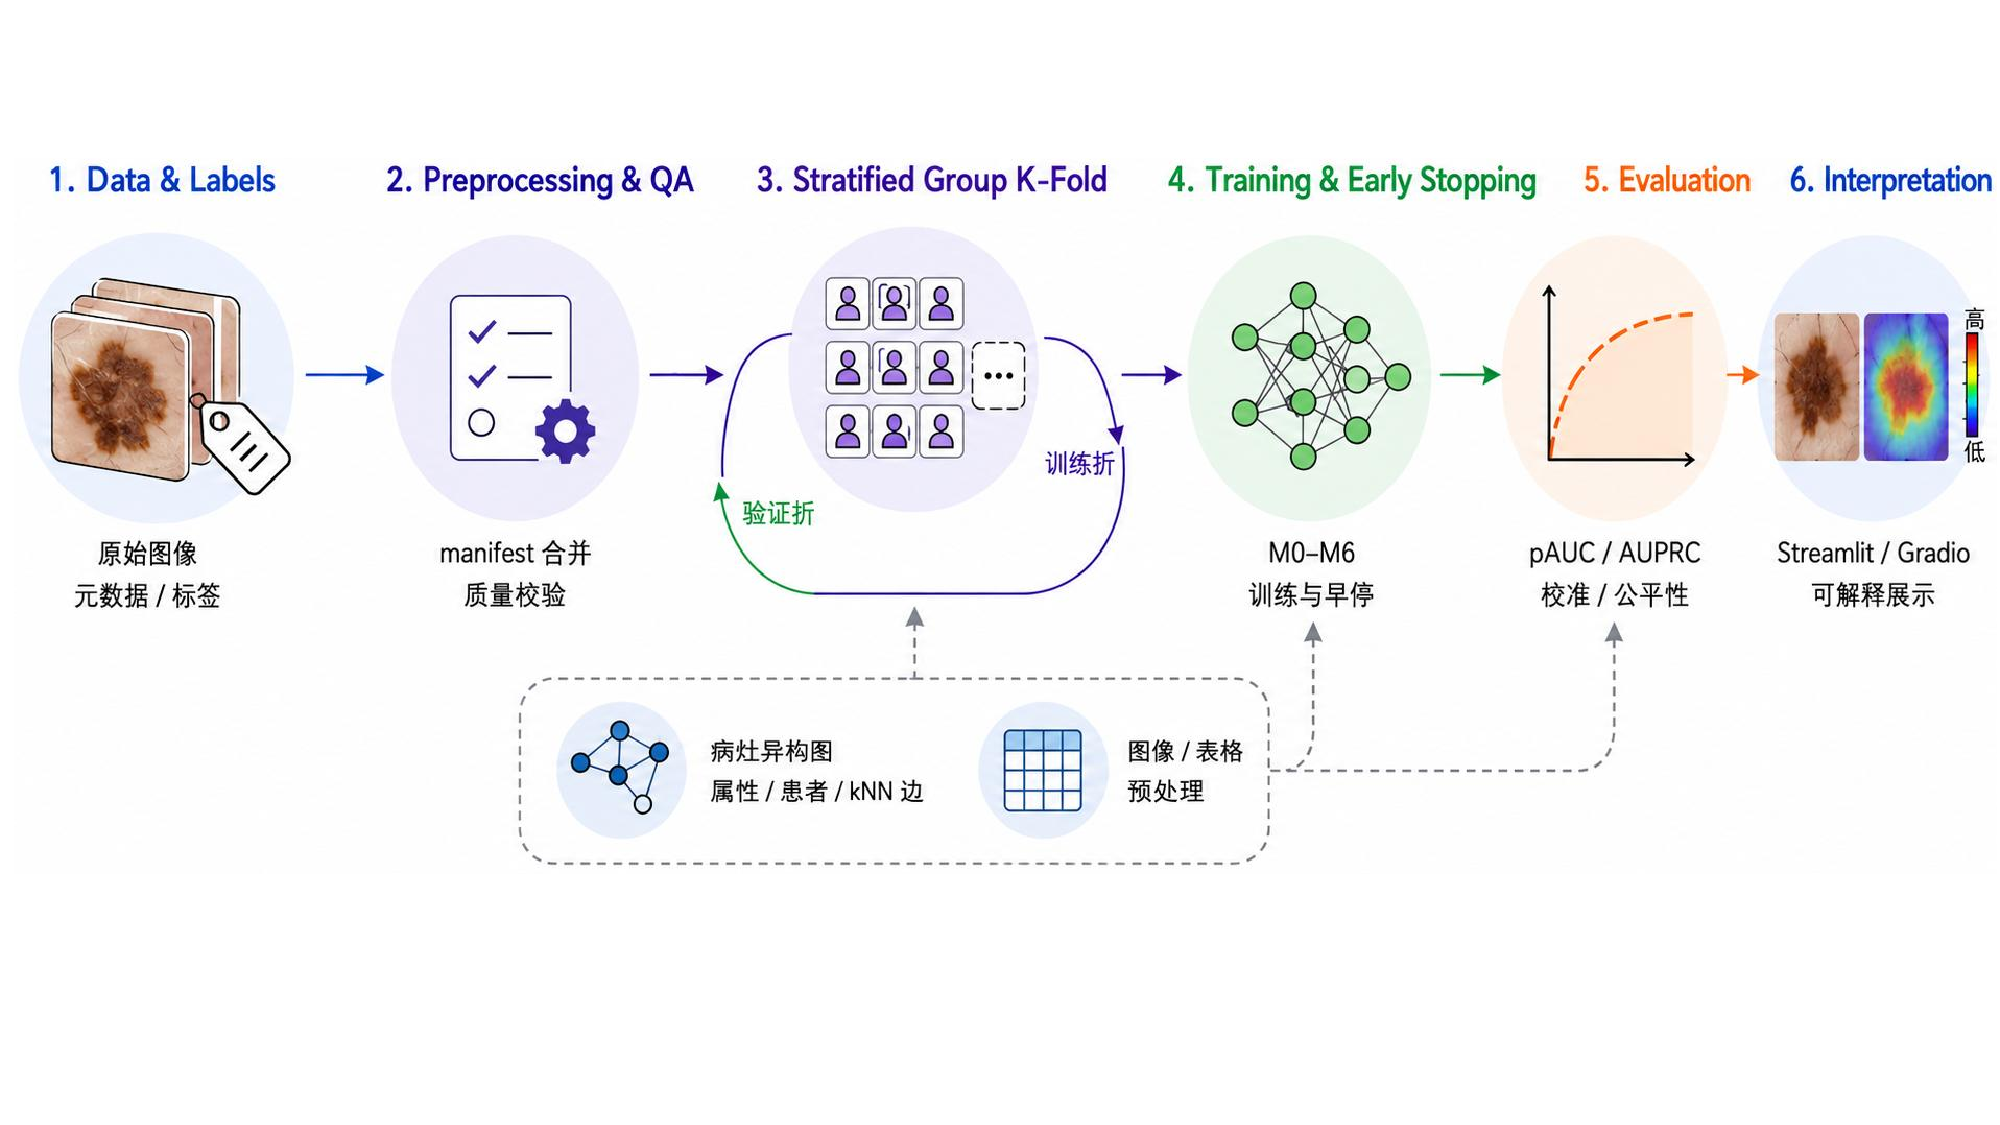
\includegraphics[width=\linewidth]{fig/ml_pipeline.pdf}
    \caption{数据处理、患者级划分、模型训练与评估流程。}
    \label{fig:ml_pipeline}
\end{figure*}
\subsection{数据来源与使用边界}
表\ref{tab:datasets} 给出本文使用的数据源。主实验仅使用 \isic{} 作为训练、验证和内部测试数据，以避免混合不同采集模态造成不可控偏差；\pad{} 用作外部验证和 Fitzpatrick 皮肤类型相关的补充分析。


\subsection{数据处理流程}
本文采用“先建清单，再分折，再按折拟合预处理器”的策略。所有均值、方差、类别词表、分箱边界、kNN 索引和图边权均在训练折上估计，然后应用到验证/测试折。

\begin{algorithm}[t]
\small
\caption{可复现数据处理流程}
\label{alg:data_pipeline}
\KwIn{原始图像目录、元数据表、标签表、配置文件 \texttt{data.yaml}}
\KwOut{manifest、fold 划分、图像索引、表格 schema、每折图边}
读取图像文件名并计算 \texttt{sample\_id}，校验图像可解码、标签唯一、元数据唯一\;
按 \texttt{sample\_id} 合并图像、元数据、补充元数据和标签，生成 \texttt{manifest\_isic.csv}\;
删除明显泄漏字段：诊断文本、活检结果、后验确认方式、目标标签的任何同义字段\;
保留 \texttt{patient\_id} 作为分组键，使用 \texttt{StratifiedGroupKFold} 构造 5 折\;
\For{每个 fold $k$}{
  仅在训练折拟合数值缺失填补、标准化、年龄/尺寸分箱、类别词表和稀有类别合并规则\;
  生成图像增强配置：训练集随机裁剪/翻转/颜色扰动，验证测试只中心缩放\;
  用训练折拟合表格预处理器并保存 \texttt{preprocessor\_foldk.pkl}\;
  构造训练图、验证/测试推理图，输出 \texttt{graph\_edges\_foldk.parquet}\;
}
对 \pad{} 执行同样 schema 对齐；不在 \isic{} 测试集上重新拟合预处理器\;
记录数据版本、文件 hash、样本数、阳性数、患者数和每折分布\;
\end{algorithm}

\subsection{图像处理}
图像模型按主干网络使用固定输入分辨率：M1 EfficientNet-B0、M2 冻结视觉编码器和 M4 ConvNeXt-Tiny 门控融合默认使用 $224\times224$，M3 Swin-Tiny 使用 $384\times384$。训练增强包括随机缩放裁剪、水平/垂直翻转、轻度亮度对比度扰动和随机擦除；验证、测试和外部验证只做确定性 resize 与中心裁剪。归一化参数采用 ImageNet 统计量或对应预训练模型要求。损坏图像、缺失图像和异常通道图像写入数据质量报告，并从可训练清单中剔除。

\subsection{元数据处理}
数值字段包括年龄、临床长径、TBP Visualizer 中的颜色/形状/位置数值特征等；类别字段包括性别、通用解剖部位和其他离散属性。处理规则如下：
\begin{itemize}
    \item 数值变量：训练折中位数填补，附加缺失指示变量，再做 robust scaling 或 z-score；
    \item 类别变量：缺失值填为 \texttt{UNK}，出现次数少于阈值 $r$ 的类别合并为 \texttt{RARE}，再使用 one-hot 或 embedding；
    \item 连续分箱：年龄按十年或五分位分箱，尺寸按训练折四分位分箱，用于图的属性节点；
    \item 禁止项：\texttt{patient\_id}、\texttt{image\_id}、\texttt{lesion\_id} 不作为普通监督特征，避免模型记忆个体或文件名。
\end{itemize}

\subsection{标签与类别不均衡处理}
\isic{} 主任务使用官方二元恶性标签。由于皮肤癌筛查数据通常极度类别不均衡，训练时记录训练折阳性率，并采用不均衡处理策略：
\begin{itemize}
    \item 损失层面：\texttt{pos\_weight}=训练折阴性数/阳性数的加权 BCE，或 Focal Loss；
    \item 采样层面：\texttt{WeightedRandomSampler} 或每个 batch 至少包含若干阳性样本；
    \item 评估层面：除 AUROC 外，同时报告 AUPRC、pAUC、固定高灵敏度阈值下的特异度、FNR 和校准误差。
\end{itemize}
\pad{} 外部验证时将 BCC、MEL、SCC/BOD 视为癌症类，将 ACK、NEV、SEK 视为非癌症类；由于采集设备、分辨率和诊断分布与 \isic{} 不同，外部结果单独成表，不与内部测试集数值直接混合平均。

\section{方法}
\begin{figure*}[t]
    \centering
    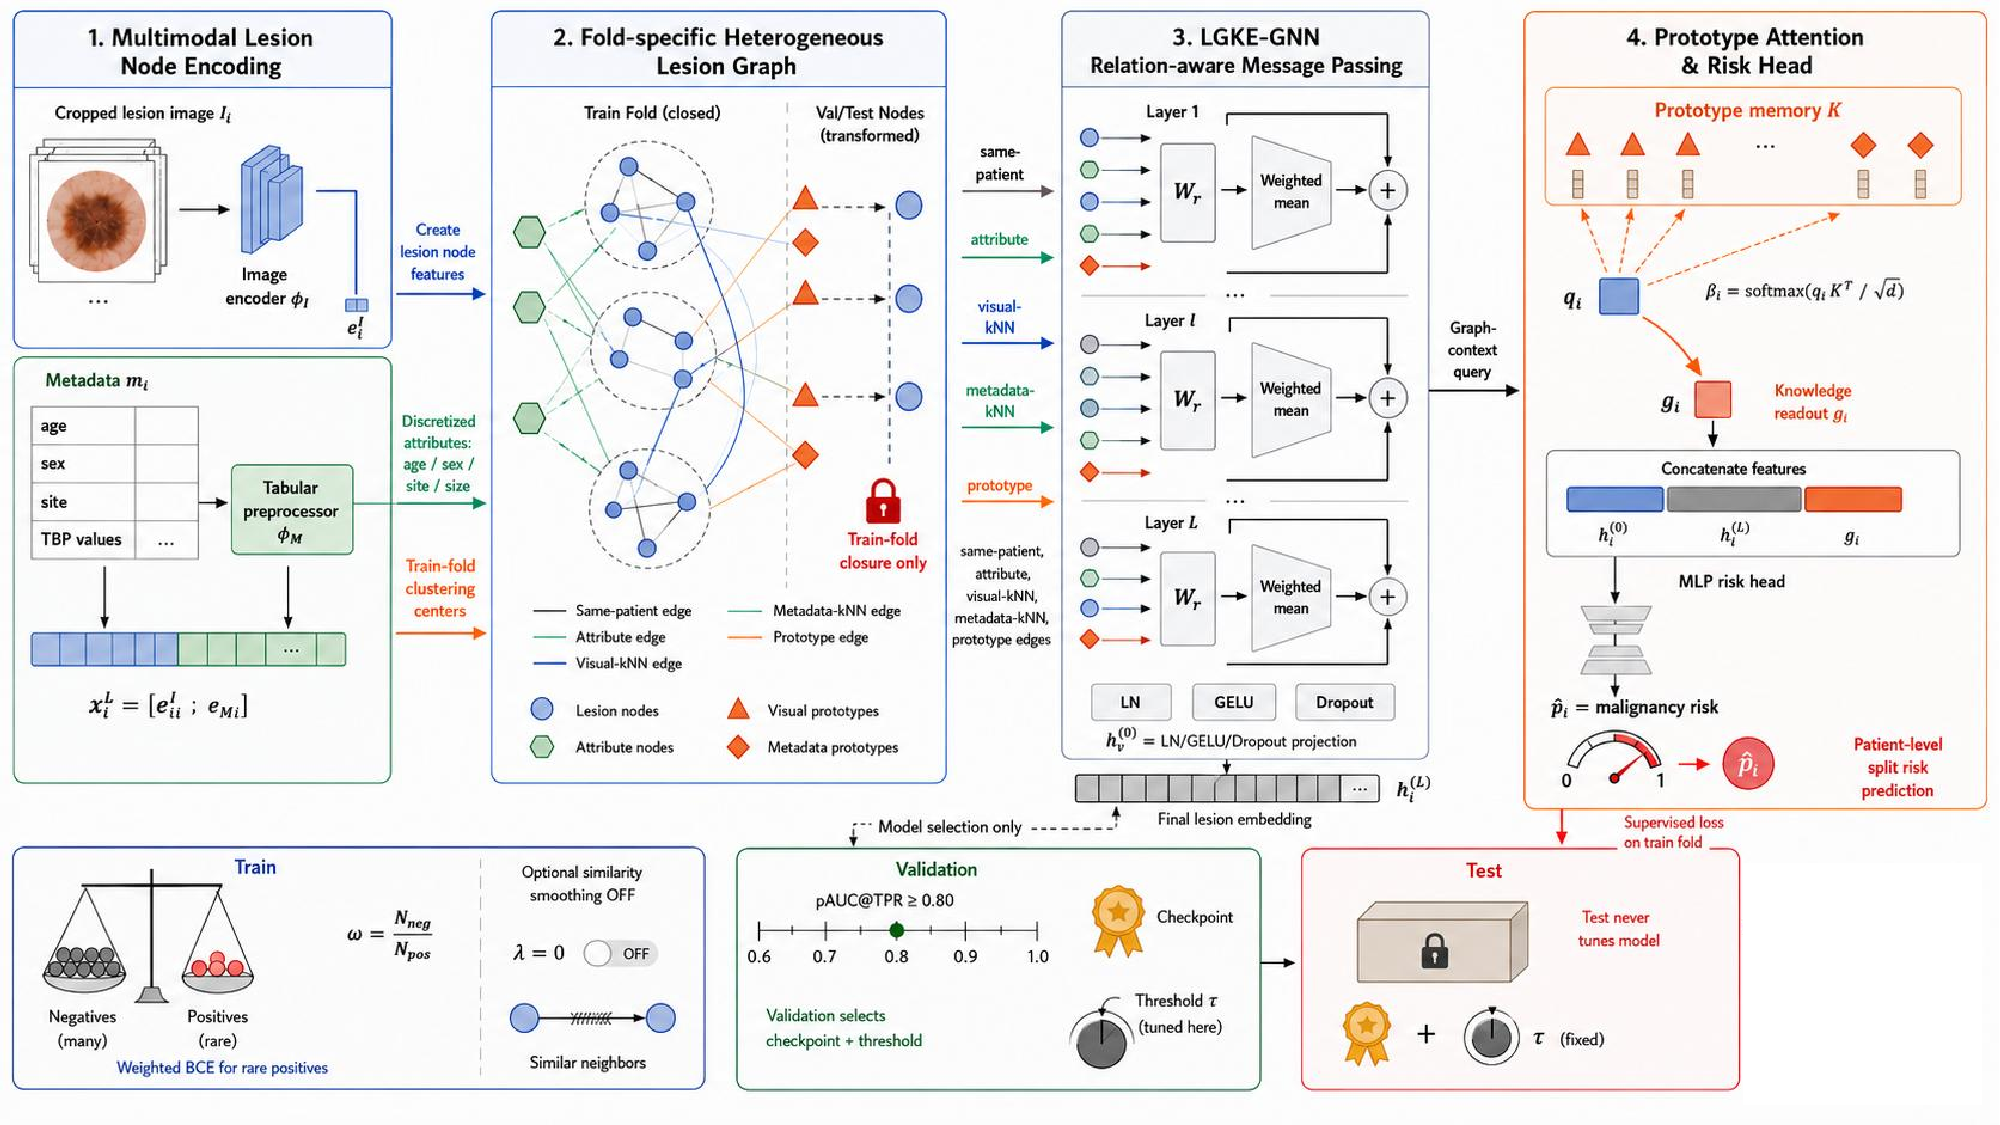
\includegraphics[width=\linewidth]{fig/m5_art.pdf}
    \caption{\modelname{} 模型架构。模型首先由图像嵌入、表格元数据和关系边构建按折划分的病灶图，然后进行关系感知图聚合与知识原型注意力读取，最终输出二分类风险分数。}
    \label{fig:arc_m5}
\end{figure*}

\subsection{任务定义与总体框架}
给定第 $i$ 个病灶样本的裁剪图像 $I_i$、结构化元数据 $m_i$、患者标识 $p_i$ 以及二元标签 $y_i\in\{0,1\}$，目标是在患者级划分下学习风险函数 $f(I_i,m_i,\mathcal{G})\rightarrow [0,1]$。与常规图像分类不同，SLICE-3D 中同一患者通常包含多个病灶，并伴随年龄、性别、解剖部位和 TBP Visualizer 数值字段。本文将这些结构性信息显式编码为异构病灶图，而非仅在样本级拼接图像和表格特征。整体框架由三部分组成：多模态节点特征编码、fold-specific 异构图构建，以及本文提出的 \modelname{} 风险编码器。

\subsection{多模态节点特征}
图像分支将病灶图像映射为向量表示 $e_i^I=\phi_I(I_i)$。正式训练使用预先缓存的图像特征，以避免在图训练阶段重复进行昂贵的视觉编码；本地调试阶段可使用轻量图像统计特征验证数据管线。元数据分支使用训练折拟合的 tabular preprocessor，对数值字段进行缺失填补、缺失指示、robust scaling，并对类别字段进行 \texttt{UNK}/\texttt{RARE} 处理。得到的元数据向量记为 $e_i^M=\phi_M(m_i)$。病灶节点的输入特征为
\begin{equation}
    x_i^L=[e_i^I;e_i^M].
\end{equation}
属性节点和原型节点同样被表示为图中的节点：属性节点对应年龄段、性别、解剖部位和尺寸分箱等离散状态；原型节点来自训练折视觉特征和元数据特征的聚类中心。所有预处理器、分箱边界、类别词表和原型均只由训练折估计。

\subsection{Fold-specific 异构病灶图}
对第 $k$ 个外层 fold，构造异构图 $\mathcal{G}^{(k)}=(\mathcal{V},\mathcal{E},\mathcal{R})$。其中 $\mathcal{V}$ 包含 lesion、attribute、visual-prototype 和 metadata-prototype 节点，$\mathcal{R}$ 包含同患者、属性、视觉近邻、元数据近邻和原型连接关系。边的构造遵循训练折闭包原则：视觉 kNN 只在训练折图像特征空间拟合，元数据 kNN 只在训练折标准化元数据空间拟合，同患者边只连接同一训练患者内部的病灶；验证和测试节点只能通过其自身特征 transform 到对应图空间，不使用标签、测试统计量或测试集调阈值信息。

对每类关系 $r\in\mathcal{R}$，邻居集合记为 $\mathcal{N}_r(i)$，边权记为 $w_{ji}^{r}$。视觉近邻边使用非负余弦相似度，元数据近邻边使用数值空间相似度，同患者边和属性边使用归一化常数权重。该图设计使模型能够同时利用三类证据：病灶自身的局部视觉形态、患者级多病灶上下文，以及训练集中稳定出现的属性和视觉相似模式。

\subsection{\modelname{} 编码器}
\modelname{} 是一个 PyTorch 原生的 relation-aware GraphSAGE 编码器。首先将所有节点特征投影到共享 hidden space：
\begin{equation}
    h_v^{(0)}=\mathrm{Dropout}\left(\mathrm{GELU}\left(\mathrm{LN}(W_0x_v)\right)\right).
\end{equation}
第 $\ell$ 层对每种关系单独变换邻居消息，并按边权加权平均：
\begin{equation}
    m_{i,r}^{(\ell)}
    =
    \frac{\sum_{j\in\mathcal{N}_r(i)} w_{ji}^{r} W_r h_j^{(\ell)}}
    {\max\left(1,\sum_{j\in\mathcal{N}_r(i)} w_{ji}^{r}\right)}.
\end{equation}
随后进行残差更新：
\begin{equation}
    h_i^{(\ell+1)}
    =
    \mathrm{LN}\left(
    h_i^{(\ell)}
    +
    \mathrm{Dropout}\left[
    \mathrm{GELU}\left(W_s h_i^{(\ell)}+\sum_{r\in\mathcal{R}}m_{i,r}^{(\ell)}\right)
    \right]\right).
\end{equation}
这种实现与标准 GraphSAGE 的局部邻域聚合一致，但保留关系类型特异的线性变换，能够区分 same-patient、attribute、visual-kNN、metadata-kNN 与 prototype 边的语义差异。

\subsection{知识原型注意力与风险头}
KGAE 的核心思想是将图结构作为共享知识空间，并通过注意力从图中读取与样本相关的知识表示 \cite{liu2021kgae}。本文不进行文本生成或报告重构，而是将这一思想转化为监督式风险筛查。设 $\mathcal{P}$ 为图中的 prototype 节点集合，最终图编码后对应矩阵为 $K=[h_p^{(L)}]_{p\in\mathcal{P}}$。对 lesion 节点 $i$，查询向量由初始表示与图上下文共同决定：
\begin{equation}
    q_i=W_q[h_i^{(0)};h_i^{(L)}],
    \qquad
    \beta_i=\mathrm{softmax}\left(\frac{q_iK^\top}{\sqrt{d}}\right),
\end{equation}
\begin{equation}
    g_i=\beta_iK.
\end{equation}
最终风险头拼接初始病灶表示、关系聚合后的图表示和原型读取向量：
\begin{equation}
    s_i=\mathrm{MLP}\left([h_i^{(0)};h_i^{(L)};g_i]\right),\qquad
    \hat{p}_i=\sigma(s_i).
\end{equation}
因此，\modelname{} 的预测不仅依赖单个病灶的多模态特征，还依赖其在患者上下文、属性空间、视觉近邻空间和原型知识空间中的相对位置。

\subsection{训练目标与模型选择}
由于阳性病灶极少，主损失使用训练折类别比例得到的加权二元交叉熵：
\begin{equation}
\mathcal{L}_{\mathrm{WBCE}}
=-\frac{1}{|\mathcal{B}|}\sum_{i\in\mathcal{B}}
\left[
\omega y_i\log \hat{p}_i+
(1-y_i)\log(1-\hat{p}_i)
\right],
\end{equation}
其中 $\omega=N_{\mathrm{neg}}/N_{\mathrm{pos}}$，并可通过 \texttt{pos\_weight\_scale} 调节。实现中保留了视觉/元数据近邻边上的可选平滑项：
\begin{equation}
    \mathcal{L}_{\mathrm{smooth}}
    =
    \lambda\sum_{(i,j)\in\mathcal{E}_{sim}}w_{ij}\|h_i^{(L)}-h_j^{(L)}\|_2^2,
\end{equation}
最终主结果使用 $\lambda=0$，以避免在极端类别不均衡条件下过度平滑阳性样本。优化器为 AdamW，模型权重由验证集 pAUC@TPR$\geq0.80$ 选择；阈值同样只在验证集上确定，并迁移到测试集。测试集不参与早停、阈值选择或超参数选择。

\subsection{比较模型}
表\ref{tab:models} 总结了用于内部患者级测试的模型族。M0--M4 覆盖表格、图像、冻结特征、Transformer 和常规多模态融合，作为评估 \modelname{} 是否真正受益于图结构的基线。

\begin{table*}[t]
\centering
\small
\caption{候选模型与实现边界。}
\label{tab:models}
\begin{tabularx}{\textwidth}{L{1.1cm}L{2.6cm}L{2.3cm}Y}
\toprule
编号 & 模型 & 输入 & 作用与关键设置 \\
\midrule
M0 & Constant prior / Metadata LightGBM & 元数据 & 建立表格基线；主结果表报告 LightGBM，constant prior 作为 sanity check \\
M1 & CNN (EfficientNet-B0) & 图像 & 建立 ImageNet 预训练 CNN 图像基线；默认输入分辨率为 $224\times224$ \\
M2 & Frozen encoder + prompt features & 图像 + 元数据文本特征 & 冻结视觉编码器，使用原始临床字段构造文本提示并提取稳定 hash 特征，再训练 MLP 分类头 \\
M3 & Transformer (Swin-Tiny) & 图像 & 检验视觉 Transformer 对 3D-TBP 裁剪图像的适配性；默认输入分辨率为 $384\times384$ \\
M4 & Gated Multimodal Fusion & 图像 + 元数据 & 使用 ConvNeXt-Tiny 图像编码器、元数据 MLP 和门控融合层进行常规多模态融合 \\
M5 & \modelname{}（KGAE-inspired） & 图像 + 元数据 + 图 & 本文方法；使用 relation-SAGE 聚合、知识原型注意力和患者级异构图上下文 \\
\bottomrule
\end{tabularx}
\end{table*}

\section{实验}
\subsection{主评估指标}
皮肤病变筛查的评价目标不同于一般二分类：模型首先需要在高灵敏度区域保持足够排序能力，以降低漏检恶性病灶的风险；同时也需要控制假阳性数量，避免给后续复查和活检带来过高负担。因此，本文不以 accuracy 作为主结论，而采用“主指标 + 辅助指标 + 阈值指标 + 校准指标”的分层评价体系。

\textbf{主指标为 pAUC@TPR$\geq0.80$。} ISIC 2024 挑战使用 TPR 高于 80\% 区间的 partial AUC 作为核心评分\cite{kaggleisic2024,isic2024challenge}。设 ROC 曲线横轴为 FPR、纵轴为 TPR，则本文只积分满足 $\mathrm{TPR}\geq0.80$ 的高灵敏度区间，并按区间宽度归一化：
\begin{equation}
    \mathrm{pAUC}_{0.80}=
    \frac{1}{1-0.80}\int_{0.80}^{1.00} \mathrm{FPR}^{-1}(t)\,dt,
\end{equation}
其中 $t$ 表示灵敏度水平，$\mathrm{FPR}^{-1}(t)$ 表示在达到该灵敏度时对应的假阳性率函数。实现时使用与 Kaggle/ISIC 口径一致的脚本计算，并在所有模型上固定同一评价函数。

\textbf{辅助排序指标包括 AUROC 与 AUPRC。} AUROC 衡量模型在全部阈值范围内区分阳性与阴性样本的能力，便于与既有研究比较；AUPRC 对阳性极少的任务更敏感，能够反映模型是否真正将恶性样本排在风险列表前部。若 AUROC 较高但 AUPRC 较低，说明模型可能主要学会区分大量阴性样本，而对少数阳性样本的排序仍不稳定。

\textbf{阈值相关指标用于模拟筛查决策。} 每个 fold 的阈值只在验证集上确定，并迁移到测试集。本文报告两组阈值：一是 Youden 指数阈值，用于观察总体平衡性能；二是验证集灵敏度不低于 90\% 的高灵敏度阈值，用于模拟筛查场景。测试集报告 Sensitivity、Specificity、FNR、FPR、F1 和 Balanced Accuracy，其中：
\begin{equation}
    \mathrm{BACC}=\frac{1}{2}\left(\frac{TP}{TP+FN}+\frac{TN}{TN+FP}\right).
\end{equation}

\textbf{校准指标用于评估风险分数可信度。} 医学筛查输出不仅需要排序正确，还需要概率分数具有可解释含义。本文报告 Brier Score、Expected Calibration Error (ECE) 和校准曲线：
\begin{equation}
    \mathrm{ECE}=\sum_{b=1}^{B}\frac{|S_b|}{n}\left|\mathrm{acc}(S_b)-\mathrm{conf}(S_b)\right|,
\end{equation}
其中 $S_b$ 为第 $b$ 个置信度分箱。ECE 越低，说明预测置信度与真实准确率越一致。所有指标均以患者级测试 fold 为单位计算均值、标准差和 bootstrap 置信区间。


\subsection{数据划分协议}
主实验使用 \texttt{StratifiedGroupKFold}，分组键为 \texttt{patient\_id}，标签为 \texttt{target}，构造 5 折患者级交叉验证。每折内训练、验证、测试的划分规则如下：
\begin{itemize}
    \item 外层测试折：每次保留约 20\% 患者作为测试集；同一患者不得跨训练与测试；
    \item 内层验证集：从剩余约 80\% 患者中再按患者级划分 10\% 作为验证集；
    \item 整体比例：由于验证集来自外层训练部分，最终每折约为 72\% 训练、8\% 验证和 20\% 测试；
    \item 模型选择：阈值、早停、超参数和集成权重只由验证集决定，测试集只用于最终评估；
    \item 外部验证：用内部最佳配置在 \isic{} 训练折重训后，直接评估 \pad{}；若进行目标域阈值重调，则作为独立实验报告。
\end{itemize}
表\ref{tab:split} 给出由 \texttt{scripts/prepare\_data.py} 自动导出的真实统计。

\begin{table}[H]
\centering
\small
\caption{患者级数据划分统计。}
\label{tab:split}
\begin{tabularx}{\columnwidth}{L{1.4cm}C{1.5cm}C{1.5cm}C{1.5cm}Y}
\toprule
数据/折 & 样本数 & 阳性数 & 患者数 & 备注 \\
\midrule
ISIC Fold 0 train & 154,204 & 209 & 456 & 训练折 \\
ISIC Fold 0 val & 19,778 & 27 & 51 & 早停和阈值 \\
ISIC Fold 0 test & 43,495 & 58 & 127 & 内部测试 \\
PAD external & 2,298 & 1,089 & 1,373 & 外部验证数据\\
\bottomrule
\end{tabularx}
\end{table}

ISIC 2024 挑战的主要评分指标为 TPR 高于 80\% 区间的 partial AUC\cite{kaggleisic2024}。因此本项目主指标设为：
\begin{itemize}
    \item \textbf{pAUC@TPR$\geq0.80$：} 与官方挑战口径对齐，强调高召回区间；
    \item \textbf{AUPRC：} 对少数阳性类别更敏感；
    \item \textbf{AUROC：} 便于与传统论文对比，但不作为唯一结论；
    \item \textbf{Sensitivity/Specificity/FNR：} 分别在 Youden 阈值和高灵敏度阈值下报告；
    \item \textbf{Brier Score 与 ECE：} 衡量风险分数校准；
    \item \textbf{推理成本：} 单张图像推理时间、显存占用、模型参数量。
\end{itemize}
Balanced Accuracy 与 ECE 定义如下：
\begin{equation}
    \mathrm{BACC}=\frac{1}{2}\left(\frac{TP}{TP+FN}+\frac{TN}{TN+FP}\right),
\end{equation}
\begin{equation}
    \mathrm{ECE}=\sum_{b=1}^{B}\frac{|S_b|}{n}\left|\mathrm{acc}(S_b)-\mathrm{conf}(S_b)\right|.
\end{equation}

\subsection{公平性指标}
设 $G$ 为性别、年龄段、解剖部位或 Fitzpatrick 类型集合。公平性分析报告：
\begin{align}
    \Delta_{\mathrm{AUC}} &= \max_{g\in G}\mathrm{AUC}_g - \min_{g\in G}\mathrm{AUC}_g,\\
    \Delta_{\mathrm{FNR}} &= \max_{g\in G}\mathrm{FNR}_g - \min_{g\in G}\mathrm{FNR}_g,\\
    \Delta_{\mathrm{ECE}} &= \max_{g\in G}\mathrm{ECE}_g - \min_{g\in G}\mathrm{ECE}_g.
\end{align}
\isic{} 主数据通常没有完整 Fitzpatrick 字段，因此 Fitzpatrick 类型主要在 \pad{} 外部验证中报告。若某子群阳性数少于预设阈值（如 10），只展示样本数和置信区间，不做强结论。

\subsection{统计显著性检验}
\begin{itemize}
    \item AUROC、AUPRC、pAUC、BACC 使用按患者 bootstrap 的 95\% 置信区间；
    \item 同一测试折上模型差异使用 paired bootstrap；AUROC 可补充 DeLong 检验；
    \item 固定阈值下的错误差异使用 McNemar 检验；
    \item 多模型多指标比较采用 Holm--Bonferroni 校正；
    \item 所有统计结论均由固定评估程序导出的 \texttt{metrics.json} 和 \texttt{stats.csv} 支撑。
\end{itemize}

\subsection{实验矩阵}
实验分为四组，避免一次性堆模型但无法解释：
\begin{enumerate}
    \item \textbf{E1 主模型对比：} M0--M6 在 5 折患者级划分下比较；
    \item \textbf{E2 融合消融：} 图像、基础元数据、TBP 数值字段、attribute nodes、visual kNN、same-patient edges 分别加入；
    \item \textbf{E3 图模型消融：} GraphSAGE vs GATv2，是否使用知识原型注意力，$K_I/K_M$ 邻居数敏感性；
    \item \textbf{E4 泛化与公平性：} 最佳内部模型在 \pad{} 上外部验证，并按 Fitzpatrick 类型、年龄、性别、部位报告差异。
\end{enumerate}



\section{结果与分析}
本节报告患者级内部测试、跨数据集泛化和子群稳定性。M0--M4 作为表格、图像和常规多模态融合基线，M5 为本文提出的 \modelname{}。除特别说明外，所有结论均基于五折患者级测试集均值与标准差；模型选择和阈值确定均在验证集完成，测试集仅用于最终评估。

\begin{figure}[t]
    \centering
    
\includegraphics[
        width=\linewidth,
        height=0.45\textheight,
        keepaspectratio
    ]{fig/main_results_forest.pdf}
\caption{各基线方法与本文 \modelname{} 在患者级内部测试集上的性能比较。点表示五折交叉验证的平均值，水平误差线表示标准差。}
    \label{fig:main_results_forest}
\end{figure}

\subsection{内部患者级测试}

% \begin{table*}[t]
% \centering
% \small
% \caption{主实验模型对比。M0--M4 为 baseline，M5 为本文提出的 Ours。所有数值均为 5 折患者级测试集均值 $\pm$ 标准差。}
% \label{tab:main_results}
% \begin{tabularx}{\textwidth}{L{1.0cm}L{2.8cm}C{1.35cm}C{1.35cm}C{1.35cm}C{1.35cm}C{1.35cm}Y}
% \toprule
% 编号 & 模型 & pAUC & AUPRC & AUROC & Sens. & Spec. & 备注 \\
% \midrule
% M0 & Metadata LightGBM
% & \makecell{0.7303\\$\pm$\\0.0737}
% & \makecell{0.0667\\$\pm$\\0.0270}
% & \makecell{0.9324\\$\pm$\\0.0168}
% & \makecell{\textbf{0.9175}\\$\pm$\\\textbf{0.0318}}
% & \makecell{0.7677\\$\pm$\\0.0604}
% & baseline；表格元数据 \\

% M1 & CNN (EfficientNet-B0)
% & \makecell{0.5408\\$\pm$\\0.0731}
% & \makecell{0.0441\\$\pm$\\0.0202}
% & \makecell{0.8734\\$\pm$\\0.0185}
% & \makecell{0.8514\\$\pm$\\0.1515}
% & \makecell{0.6537\\$\pm$\\0.1756}
% & baseline；图像 CNN \\

% M2 & MONET Feature
% & \makecell{0.5892\\$\pm$\\0.0837}
% & \makecell{0.0409\\$\pm$\\0.0192}
% & \makecell{0.8826\\$\pm$\\0.0265}
% & \makecell{0.7942\\$\pm$\\0.0667}
% & \makecell{0.8089\\$\pm$\\0.0438}
% & baseline；冻结视觉特征 \\

% M3 & Transformer (Swin-Tiny)
% & \makecell{0.6418\\$\pm$\\0.0653}
% & \makecell{0.0471\\$\pm$\\0.0124}
% & \makecell{0.9011\\$\pm$\\0.0232}
% & \makecell{0.8486\\$\pm$\\0.0743}
% & \makecell{0.7756\\$\pm$\\0.0862}
% & baseline；视觉 Transformer \\

% M4 & Late/Gated Fusion
% & \makecell{0.7393\\$\pm$\\0.0741}
% & \makecell{\textbf{0.0765}\\$\pm$\\\textbf{0.0487}}
% & \makecell{0.9328\\$\pm$\\0.0188}
% & \makecell{0.8678\\$\pm$\\0.0552}
% & \makecell{\textbf{0.8445}\\$\pm$\\\textbf{0.0953}}
% & baseline；门控多模态融合 \\

% M5 & \modelname{}
% & \makecell{\textbf{0.7794}\\$\pm$\\\textbf{0.0748}}
% & \makecell{0.0708\\$\pm$\\0.0397}
% & \makecell{\textbf{0.9415}\\$\pm$\\\textbf{0.0160}}
% & \makecell{0.9088\\$\pm$\\0.0529}
% & \makecell{0.8129\\$\pm$\\0.0778}
% & \textbf{Ours}；图结构多模态模型 \\
% \bottomrule
% \end{tabularx}
% \end{table*}

\begin{table*}[t]
\centering
\small
\renewcommand{\arraystretch}{1.22}
\setlength{\tabcolsep}{3pt}
\caption{主实验模型对比。M0--M4 为基线模型，M5 为本文提出的方法。所有指标均以百分比展示，数值为 5 折患者级测试集均值 $\pm$ 标准差。}
\label{tab:main_results}

\begin{tabular*}{\textwidth}{@{\extracolsep{\fill}}llccccc}
\toprule
编号 & 模型 & pAUC (\%) & AUPRC (\%) & AUROC (\%) & Sens. (\%) & Spec. (\%) \\
\midrule
M0 & Metadata LightGBM
& \mbox{73.03 $\pm$ 7.37}
& \mbox{6.67 $\pm$ 2.70}
& \mbox{93.24 $\pm$ 1.68}
& \mbox{\textbf{91.75 $\pm$ 3.18}}
& \mbox{76.77 $\pm$ 6.04} \\

M1 & CNN (EfficientNet-B0)
& \mbox{54.08 $\pm$ 7.31}
& \mbox{4.41 $\pm$ 2.02}
& \mbox{87.34 $\pm$ 1.85}
& \mbox{85.14 $\pm$ 15.15}
& \mbox{65.37 $\pm$ 17.56} \\

M2 & MONET Feature
& \mbox{58.92 $\pm$ 8.37}
& \mbox{4.09 $\pm$ 1.92}
& \mbox{88.26 $\pm$ 2.65}
& \mbox{79.42 $\pm$ 6.67}
& \mbox{80.89 $\pm$ 4.38} \\

M3 & Transformer (Swin-Tiny)
& \mbox{64.18 $\pm$ 6.53}
& \mbox{4.71 $\pm$ 1.24}
& \mbox{90.11 $\pm$ 2.32}
& \mbox{84.86 $\pm$ 7.43}
& \mbox{77.56 $\pm$ 8.62} \\

M4 & Late/Gated Fusion
& \mbox{\underline{73.93 $\pm$ 7.41}}
& \mbox{\textbf{7.65 $\pm$ 4.87}}
& \mbox{\underline{93.28 $\pm$ 1.88}}
& \mbox{86.78 $\pm$ 5.52}
& \mbox{\textbf{84.45 $\pm$ 9.53}} \\

M5 & \modelname{}
& \mbox{\textbf{77.94 $\pm$ 7.48}}
& \mbox{\underline{7.08 $\pm$ 3.97}}
& \mbox{\textbf{94.15 $\pm$ 1.60}}
& \mbox{\underline{90.88 $\pm$ 5.29}}
& \mbox{\underline{81.29 $\pm$ 7.78}} \\
\bottomrule
\end{tabular*}
\end{table*}

\modelname{} 在主指标 pAUC@TPR$\geq0.80$ 上取得最高结果，达到 $77.94\pm7.48$，相较最强 baseline M4 提升 4.01 个百分点。AUROC 也达到 $94.15\pm1.60$，表明患者上下文、属性关系和视觉近邻关系能够提升整体风险排序能力。AUPRC 方面，M5 为 $7.08\pm3.97$，低于 M4 的 $7.65\pm4.87$ 但显著高于图像单模态模型，说明在极端类别不均衡场景中，普通门控融合仍是强少数类排序基线，而图结构主要贡献体现在高灵敏度区间和总体判别性能。M0 的 sensitivity 最高，但 specificity 明显低于 M4 和 M5，提示仅提升召回率会引入更多假阳性。综合 pAUC、AUROC、sensitivity 和 specificity，\modelname{} 在内部患者级筛查设定下给出了更均衡的风险筛查性能。

\begin{figure*}[t]
    \centering
    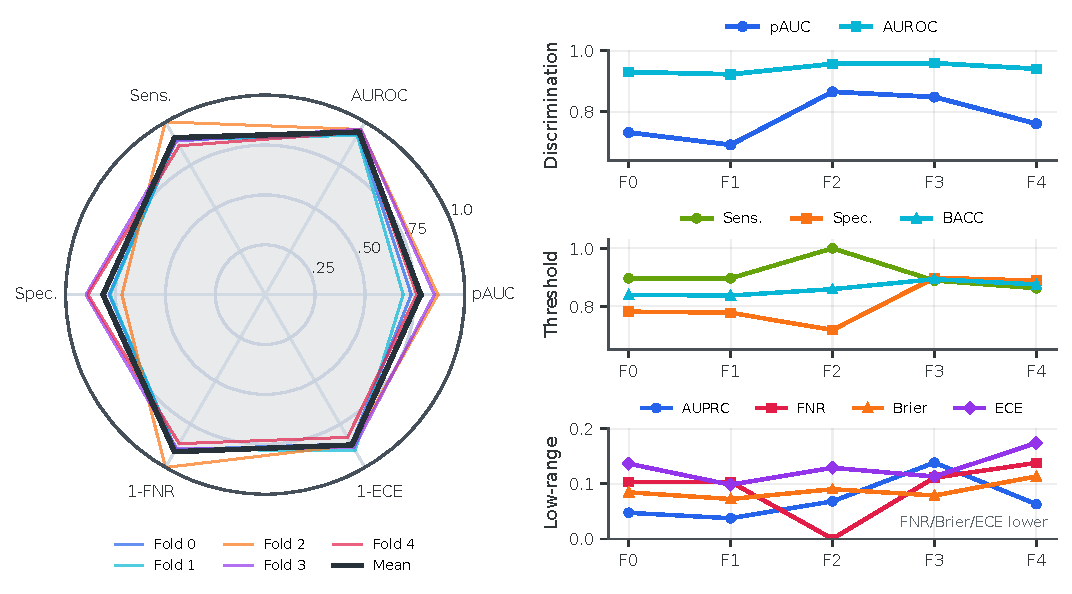
\includegraphics[width=\textwidth]{fig/m5_fold_profile.pdf}
\caption{\modelname{} 的五折表现。雷达图采用“数值越大表示表现越好”的指标方向，其中 FNR 和 ECE 分别显示为 $1-\mathrm{FNR}$ 和 $1-\mathrm{ECE}$。右侧子图以折线形式展示判别指标（pAUC 与 AUROC）以及错误/校准指标（FNR 与 ECE）的折间变化。}
    \label{fig:m5_fold_profile}
\end{figure*}

图\ref{fig:m5_fold_profile} 展示了 \modelname{} 的折间稳定性。AUROC 在五折中均维持在较高水平，而 pAUC 的波动更明显，反映出高灵敏度区间对阳性样本数量和 fold 难度更敏感。FNR 在第 2 折最低，在第 4 折相对较高；ECE 的变化也表明不同测试折存在校准差异。因此，M5 的优势不能仅由单折结果解释，而应理解为在患者级五折协议下对高灵敏度排序、漏诊控制和校准稳定性的综合折中。

\subsection{跨数据集泛化}
\begin{table}[H]
\centering
\footnotesize
\renewcommand{\arraystretch}{1.25}
\setlength{\tabcolsep}{3pt}
\caption{跨数据集外部验证。所有指标均以百分比展示，数值为 5 折患者级测试集均值 $\pm$ 标准差。}
\label{tab:external}

\begin{tabular*}{\columnwidth}{@{\extracolsep{\fill}}lccc}
\toprule
训练/测试设置 & AUPRC (\%) & AUROC (\%) & BACC (\%) \\
\midrule
\makecell[l]{ISIC 训练\\ISIC 测试}
& \mbox{77.94 $\pm$ 7.48}
& \mbox{94.15 $\pm$ 1.60}
& \mbox{86.08 $\pm$ 2.41} \\

\makecell[l]{ISIC 训练\\PAD 测试}
& \mbox{48.85 $\pm$ 16.97}
& \mbox{47.35 $\pm$ 26.64}
& \mbox{41.29 $\pm$ 13.53} \\

\makecell[l]{ISIC 预训练\\ PAD fine-tune}
& \mbox{77.48 $\pm$ 5.01}
& \mbox{85.47 $\pm$ 3.09}
& \mbox{81.25 $\pm$ 2.51} \\
\bottomrule
\end{tabular*}

\vspace{2pt}
\begin{minipage}{\columnwidth}
\scriptsize
\textit{注：}
ISIC 训练、ISIC 测试为内部患者级测试，采用 M5 high-sensitivity threshold；
ISIC 训练、PAD 测试为零样本外部迁移，未在 PAD 上调阈值；
ISIC 预训练 + PAD-only fine-tune 表示 PAD 患者级 5 折目标域适配。
\end{minipage}
\end{table}

\begin{figure}[H]
    \centering
    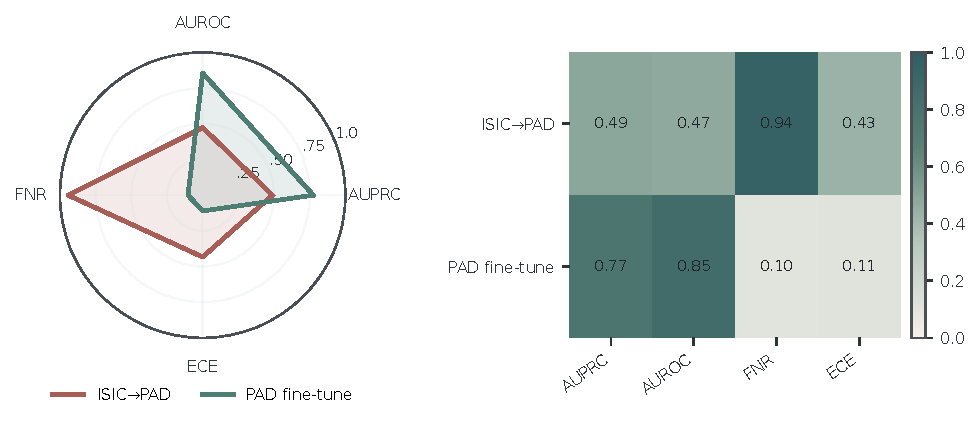
\includegraphics[width=\columnwidth]{fig/pad_domain_shift.pdf}
    \caption{在PAD-UFES-20上测试外部域的行为。直接从ISIC迁移存在严重的阈值和校准偏移问题，而目标域微调则能恢复判别性和高灵敏度性能。}
    \label{fig:pad_domain_shift}
\end{figure}

\pad{} 外部验证显示出显著域迁移。直接将 ISIC 训练模型应用到 PAD 时，AUROC 降至 $47.35\pm26.64$，balanced accuracy 仅为 $41.29\pm13.53$；这表明 3D-TBP 裁剪图像与智能手机临床照片之间存在明显采集域差异，且 ISIC 验证集阈值不能直接迁移到 PAD。相比之下，PAD-only fine-tune 将 AUROC 提升至 $85.47\pm3.09$，balanced accuracy 提升至 $81.25\pm2.51$。该结果说明，\modelname{} 的结构在目标域具备标注样本时能够完成有效适配，但零样本外部泛化仍然不足。后续部署应优先研究域鲁棒预训练、目标域校准和阈值迁移，而不是直接将内部测试性能外推到临床手机图像域。

\subsection{公平性评估结果}

% \begin{table}[t]
% \centering
% \small
% \setlength{\tabcolsep}{2pt}
% \renewcommand{\arraystretch}{0.95}
% \caption{子群公平性评估结果。表中报告不同子群的样本数、阳性样本数及分类性能指标。对于阳性样本数较少的子群，相关指标仅作描述性参考，不作强结论。部位缩写：ant.=anterior, post.=posterior, ext.=extremity。}
% \label{tab:fairness}
% \begin{tabular}{@{}llrrrrr@{}}
% \toprule
% 分组变量 & 子群 & 样本数 & 阳性数 & AUROC & Sens. & FNR \\
% \midrule
% 性别 & UNK & 2,319 & 5 & 0.8971 & 0.6000 & 0.4000 \\
% 性别 & female & 61,986 & 68 & 0.8978 & 0.8382 & 0.1618 \\
% 性别 & male & 153,172 & 221 & 0.9445 & 0.9367 & 0.0633 \\

% 年龄 & $<40$ & 16,363 & 6 & 0.9124 & 0.6667 & 0.3333 \\
% 年龄 & 40--59 & 77,975 & 78 & 0.9282 & 0.8846 & 0.1154 \\
% 年龄 & 60--79 & 109,754 & 180 & 0.9318 & 0.9222 & 0.0778 \\
% 年龄 & $\geq 80$ & 12,180 & 29 & 0.9449 & 0.9310 & 0.0690 \\
% 年龄 & UNK & 1,205 & 1 & 0.9925 & 1.0000 & 0.0000 \\

% 部位 & ant. torso & 46,827 & 54 & 0.9011 & 0.8889 & 0.1111 \\
% 部位 & head/neck & 5,924 & 65 & 0.8545 & 0.9846 & 0.0154 \\
% 部位 & lower ext. & 57,272 & 63 & 0.9353 & 0.8730 & 0.1270 \\
% 部位 & post. torso & 65,272 & 68 & 0.9367 & 0.9118 & 0.0882 \\
% 部位 & upper ext. & 38,686 & 44 & 0.9235 & 0.8636 & 0.1364 \\
% \bottomrule
% \end{tabular}
% \end{table}

\begin{table*}[t]
\centering
\footnotesize
\setlength{\tabcolsep}{4.2pt}
\renewcommand{\arraystretch}{1.08}
\caption{子群公平性评估结果。表中报告不同子群的样本数、阳性样本数及分类性能指标。对于阳性样本数较少的子群，相关指标仅作描述性参考，不作强结论。部位缩写沿用原始字段：ant. 表示前躯干，post. 表示后躯干，ext. 表示肢体。}
\label{tab:fairness}

\begin{minipage}[t]{0.47\textwidth}
\vspace{0pt}
\centering
\begin{tabular}[t]{@{}llrrrr@{}}
\toprule
分组 & 子群 & 样本/阳性 & AUROC & Sens. & FNR \\
\midrule
\multicolumn{6}{@{}l}{\textbf{性别}} \\
性别 & UNK    & 2,319 / 5     & 0.8971 & 0.6000 & 0.4000 \\
性别 & female & 61,986 / 68   & 0.8978 & 0.8382 & 0.1618 \\
性别 & male   & 153,172 / 221 & 0.9445 & 0.9367 & 0.0633 \\

\midrule
\multicolumn{6}{@{}l}{\textbf{年龄}} \\
年龄 & $<40$    & 16,363 / 6    & 0.9124 & 0.6667 & 0.3333 \\
年龄 & 40--59   & 77,975 / 78   & 0.9282 & 0.8846 & 0.1154 \\
年龄 & 60--79   & 109,754 / 180 & 0.9318 & 0.9222 & 0.0778 \\
年龄 & $\geq 80$ & 12,180 / 29  & 0.9449 & 0.9310 & 0.0690 \\
年龄 & UNK      & 1,205 / 1     & 0.9925 & 1.0000 & 0.0000 \\
\bottomrule
\end{tabular}
\end{minipage}
\hfill
\begin{minipage}[t]{0.49\textwidth}
\vspace{0pt}
\centering
\begin{tabular}[t]{@{}llrrrr@{}}
\toprule
分组 & 子群 & 样本/阳性 & AUROC & Sens. & FNR \\
\midrule
\multicolumn{6}{@{}l}{\textbf{部位}} \\
部位 & ant. torso  & 46,827 / 54 & 0.9011 & 0.8889 & 0.1111 \\
部位 & head/neck   & 5,924 / 65  & 0.8545 & 0.9846 & 0.0154 \\
部位 & lower ext.  & 57,272 / 63 & 0.9353 & 0.8730 & 0.1270 \\
部位 & post. torso & 65,272 / 68 & 0.9367 & 0.9118 & 0.0882 \\
部位 & upper ext.  & 38,686 / 44 & 0.9235 & 0.8636 & 0.1364 \\
\bottomrule
\end{tabular}

\vspace{0.8em}

\begin{tabular}{@{}p{0.96\linewidth}@{}}
\toprule
\textbf{简要观察} \\
\midrule
性别维度中，male 子群的 AUROC 和召回率较高，female 子群 FNR 相对更高。年龄维度中，$<40$ 与 UNK 子群阳性样本数很少，因此指标仅作描述性参考。部位维度中，head/neck 子群召回率最高但 AUROC 较低，upper ext. 和 lower ext. 的 FNR 相对较高。 \\
\bottomrule
\end{tabular}
\end{minipage}

\end{table*}

子群结果表明，模型在性别、年龄段和解剖部位之间存在非均匀表现。male 子群的 AUROC 和召回率较高，而 female 子群 FNR 更高；年龄维度中，$<40$ 与 UNK 子群阳性样本数很少，指标不应被解释为稳定估计；部位维度中，head/neck 子群召回率较高但 AUROC 较低，upper extremity 和 lower extremity 的 FNR 相对更高。由于若干子群阳性样本不足，本文将这些差异视为需要进一步验证的公平性风险信号，而非确定性偏见结论。外部 PAD 结果还提示，跨域阈值迁移失败可能放大子群 FNR，因此公平性评估应与域适配和校准迁移共同考虑。

\section{作者贡献}
表\ref{tab:roles} 概述团队成员在数据处理、模型实现、评估分析和系统整理中的主要贡献。该表用于说明研究工作的组织方式，不参与模型性能比较。

\begin{table*}[h]
\centering
\small
\caption{作者贡献概述。}
\label{tab:roles}
\begin{tabularx}{\textwidth}{L{3.0cm}L{2.1cm}Y Y}
\toprule
模块 & 成员 & 主要贡献 & 研究产出 \\
\midrule
数据管线、图构建与基线多模态模型 
& 郝哲逸 
& 构建统一 manifest、图像质量检查、患者级五折划分、元数据预处理器和图结构中间表示；实现并训练 M0--M4 基线。
& 形成患者级数据管线、基线模型结果和主实验比较表。 \\
\midrule
图神经网络模型与消融分析
& 林青滢 
& 设计并实现 \modelname{} 的关系聚合、知识原型注意力、训练流程和图结构消融实验。
& 形成 M5 主结果、图结构消融、训练诊断和结构级解释性分析。 \\
\midrule
评估、公平性与统计分析
& 高文昊 
& 实现 pAUC、AUPRC、AUROC、Brier score、ECE、患者级 bootstrap 和子群公平性分析。
& 形成统一评估协议、外部验证分析、公平性表和论文图表。 \\
\midrule
实验整理与可复现材料 
& 姜政言 
& 整理运行环境、实验入口、报告素材和展示材料，协助复现实验流程与结果归档。
& 形成可复现实验说明、环境配置和结果展示材料。 \\
\bottomrule
\end{tabularx}
\end{table*}

\section{讨论}

\textbf{1）关于 LGKE-GNN 的有效性。}
内部患者级测试结果表明，\modelname{} 在 pAUC@TPR$\geq0.80$ 与 AUROC 上优于表格、图像和常规多模态 baseline，说明病灶图结构能够为高灵敏度筛查提供额外信息。其优势主要来自两个方面：第一，同患者边和视觉近邻边使模型能够利用 patient-level context，近似临床中的 ``ugly duckling'' 比较逻辑；第二，知识原型注意力将分散的属性组合与视觉聚类模式压缩为全局可读取模板，缓解了单个 batch 或局部子图信息不足的问题。需要注意的是，\modelname{} 并非在所有指标上绝对占优，例如 AUPRC 与门控融合 M4 的差距很小，这提示图结构主要改善高灵敏度区间排序和总体判别能力，而少数类精确排序仍需要更强的阳性样本建模。

\textbf{2）关于类别不均衡与指标解释。}
\isic{} 中恶性样本占比极低，accuracy 在该任务中几乎没有解释力，AUROC 也可能在大量阴性样本主导下显得偏乐观。因此本文将 pAUC、AUPRC、FNR、specificity 和校准指标联合报告。特别是在筛查场景中，灵敏度提高通常伴随假阳性增加；如果只报告最高 sensitivity，模型可能通过牺牲 specificity 获得表面优势。本文采用验证集高灵敏度阈值并迁移到测试集，是为了避免在测试集上调阈值导致乐观偏差。

\textbf{3）关于跨域泛化。}
外部验证显示，直接将 ISIC 训练模型迁移到 \pad{} 时性能明显下降，而 PAD-only fine-tune 能显著恢复 AUROC、BACC 和 FNR。这一现象说明模型并未学习到完全域不变的皮肤病变表示。\isic{} 的图像来自 3D-TBP 裁剪，\pad{} 则来自智能手机临床照片，两者在视角、光照、分辨率、背景和标签分布上均存在差异。因此，外部验证下降不能简单解释为模型结构失败，更应被视为采集域迁移和阈值迁移共同作用的结果。后续工作可引入域自适应训练、目标域少样本校准、图像风格归一化和测试时阈值校准，以提升跨设备部署稳定性。

\textbf{4）关于公平性结论的边界。}
性别、年龄段和解剖部位的子群结果显示出可见差异，但部分子群阳性样本数很少，置信区间会非常宽。在这种情况下，本文不将单个子群指标差异直接解释为确定性偏见，而将其作为需要进一步收集数据和复核的风险信号。Fitzpatrick 类型也并不等同于真实肤色或族群身份，其标注可能存在主观性和缺失性；因此 PAD 上的皮肤类型分析仅能作为公平性补充证据，不能替代更系统的肤色、多中心和多设备评估。

\textbf{5）关于图结构的潜在风险。}
病灶图虽然能引入上下文，但也可能放大数据偏差。例如，如果某些患者、部位或视觉簇中阳性比例异常，模型可能过度依赖图邻居而非病灶本身；如果图边在全数据上构造，则会发生严重信息泄漏。本文通过 fold-specific 图构建、训练折拟合 kNN、限制同患者邻居数和图结构消融来降低这些风险。未来还应进一步分析边类型贡献、错误样本的 Top-$k$ 邻居、知识原型注意力分布和不同子群中的图依赖强度。

\textbf{6）医学应用限制与未来方向。}
本系统仅用于课程研究和方法验证，不能用于临床诊断或替代医生判断。真实部署还需要前瞻性验证、跨医院数据、设备标准化、医生-in-the-loop 工作流、隐私合规和可解释性审查。后续研究可从四个方向扩展：其一，使用自监督或医学基础模型提升 3D-TBP 图像编码质量；其二，引入域泛化和校准迁移以改善 PAD 等外部域表现；其三，构建更细粒度的病灶图解释模块，使模型输出能够说明关键邻居和属性证据；其四，在更多肤色、年龄和采集设备子群上验证公平性与鲁棒性。

\section{结论}
本文围绕皮肤病变筛查任务提出 \modelname{}，将病灶图像、临床元数据、患者上下文、属性节点和视觉近邻关系统一到异构图表示中。在 ISIC 患者级五折测试中，\modelname{} 在主指标 pAUC@TPR$\geq0.80$ 上达到 $0.7794\pm0.0748$，AUROC 达到 $0.9415\pm0.0160$，并在本轮种子聚焦训练中将 AUPRC 提升至 $0.0708\pm0.0397$。这些结果表明，\modelname{} 在高灵敏度筛查区间和整体排序性能上优于本研究实现的表格、图像和常规多模态 baseline。外部 PAD 结果表明，零样本跨域迁移仍然脆弱，但 PAD 目标域微调能显著恢复目标域性能。总体而言，\modelname{} 在内部患者级筛查场景中具有较强判别能力；未来工作应优先改进跨域鲁棒性、目标域校准和小样本子群稳定性。

\appendix

\section{\modelname{} 实现细节、训练诊断与解释性分析}

\subsection{张量接口与模块分解}
\modelname{} 的实现位于 \texttt{src/skin\_lesion\_risk/models/adapters/graph.py}。输入图以 PyTorch tensor 字典表示，核心字段包括节点特征 \texttt{x}、边索引 \texttt{edge\_index}、边类型 \texttt{edge\_type}、边权 \texttt{edge\_weight}、病灶节点索引 \texttt{lesion\_indices} 以及训练/评估掩码。该设计避免依赖 PyG，使本地调试和 CUDA 训练共享同一套执行路径。模型由四个连续模块组成：输入投影、关系特异 GraphSAGE 聚合、知识原型注意力和二分类风险头。

\begin{table}[H]
\centering
\small
\caption{\modelname{} 关键模块与实现边界。}
\label{tab:appendix_m5_modules}
\begin{tabularx}{\columnwidth}{L{2.2cm}Y}
\toprule
模块 & 设计说明 \\
\midrule
图像投影器 & 将冻结或缓存的图像特征投影到共享隐空间 \\
元数据编码器 & 数值变量经缺失填补与尺度归一化，类别变量经折内词表后编码 \\
异构关系聚合 & 对同患者、属性、视觉 kNN、元数据 kNN、原型等关系分别进行线性变换、边权归一化聚合和残差更新 \\
知识原型注意力 & 使用视觉与元数据原型节点作为可读取的知识槽，补充局部邻域外的全局模式 \\
风险预测头 & 拼接初始病灶表示、图上下文和原型读取向量，输出二分类风险 logit \\
训练目标 & 加权 BCE，正类权重由训练折阴阳性比例决定；早停指标为验证集 pAUC \\
\bottomrule
\end{tabularx}
\end{table}

\noindent\textbf{模块分析。}
表\ref{tab:appendix_m5_modules} 展示了 \modelname{} 的实现边界。图像投影器和元数据编码器分别承担模态对齐功能，使异构输入能够进入同一隐空间；关系聚合层则是区别于普通后期融合的核心部分，它对不同边类型使用独立线性变换，从而避免将“同患者上下文”“属性共现”和“视觉相似性”混为同一类邻居证据。知识原型注意力提供的是全局模式读取，而不是局部邻域的重复聚合；这使模型在阳性样本稀少、单个批次中恶性样本不足时，仍能访问训练折中学习到的视觉和元数据原型。风险预测头拼接三类表示，能够同时保留病灶自身特征、图上下文特征和原型读取特征。

\subsection{关键超参数}
最终主结果采用种子聚焦超参数搜索中综合表现最稳定的配置：隐空间维度 128、2 层图聚合、学习率 $1.8\times10^{-4}$、dropout 0.15、早停耐心 18，随机种子为 9701。五折训练日志显示，最佳验证集 pAUC 分别出现在第 61、102、105、99 和 75 个训练轮次；所有模型权重均由验证集 pAUC@TPR$\geq0.80$ 选择，测试集仅用于最终报告。正式训练在 NVIDIA GeForce RTX 5090 GPU 上完成，使用 CUDA 后端执行图张量计算；本地机器仅用于数据管线检查、CPU 级别连通性验证和报告生成，不用于报告主结果训练。表\ref{tab:appendix_hparams} 汇总了主配置，图\ref{fig:m5_sweep} 给出超参数敏感性。

\begin{table}[H]
\centering
\small
\caption{主结果中 \modelname{} 的训练配置。}
\label{tab:appendix_hparams}
\begin{tabularx}{\columnwidth}{L{2.5cm}Y}
\toprule
项目 & 设置 \\
\midrule
隐空间维度 & 128 \\
图聚合层数 & 2 \\
原型节点数 & 128 \\
视觉 kNN / 元数据 kNN & 10 / 10 \\
优化器 & AdamW \\
学习率 & $1.8\times10^{-4}$ \\
权重衰减 & $1\times10^{-4}$ \\
Dropout & 0.15 \\
最大轮数 / 早停耐心 & 110 / 18 \\
随机种子 & 9701 \\
训练硬件 & NVIDIA GeForce RTX 5090 GPU（CUDA） \\
损失函数 & 基于训练折正类权重的加权 BCE \\
早停准则 & 验证集 pAUC@TPR$\geq0.80$ \\
阈值选择 & 验证集高灵敏度阈值迁移到测试集 \\
划分协议 & StratifiedGroupKFold，患者级划分，5 折 \\
\bottomrule
\end{tabularx}
\end{table}

\noindent\textbf{配置分析。}
最终配置没有继续扩大隐空间维度，而是保持 128 维隐空间和 2 层关系聚合。这一选择主要基于两点考虑：首先，图中病灶节点数远大于阳性节点数，过大的隐空间容易在训练折中继续降低加权 BCE，却未必提升高灵敏度区间排序；其次，2 层聚合已经可以覆盖一阶关系节点和二阶局部上下文，再增加层数会提高过平滑风险。学习率 $1.8\times10^{-4}$ 与 dropout 0.15 在训练稳定性和 AUPRC 之间提供了更好的折中。早停耐心 18 允许后期 pAUC 继续改善，避免过早停止；但模型选择仍严格由验证集决定，测试折不参与任何阈值或权重选择。

\begin{figure*}[t]
    \centering
    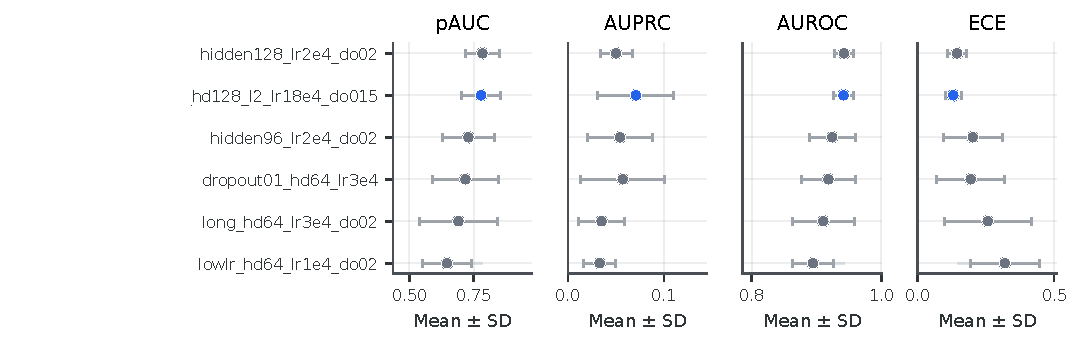
\includegraphics[width=\textwidth]{fig/m5_hparam_sweep.pdf}
\caption{\modelname{} 的超参数敏感性分析。最终采用的种子聚焦配置在保持具有竞争力的 pAUC 和 AUROC 的同时，相较于早期仅以 pAUC 为优化目标的配置，进一步提升了 AUPRC 和校准性能。}
    \label{fig:m5_sweep}
\end{figure*}

图\ref{fig:m5_sweep} 表明，早期仅优化 pAUC 的配置在主指标上非常接近最终配置，但 AUPRC 和 ECE 不够理想。最终种子聚焦配置的 pAUC 略低于早期单指标最优点，但 AUPRC 明显提高，ECE 也更低；这与本文的筛查目标更一致，因为临床风险排序不能只关注高灵敏度区间的 ROC 面积，还需要保证少数阳性样本在风险列表前端具有更好的集中度，并减少概率输出的校准偏移。因此，最终模型选择采用综合指标而非单一 pAUC 最大化。

\subsection{LGKE-GNN 训练动态}
图\ref{fig:m5_training_diagnostics} 仅使用 LGKE-GNN 的真实训练日志，比较最终种子聚焦配置与早期仅优化 pAUC 的配置。两组模型的训练损失均持续下降，而验证损失在中后期出现回升，说明图模型在极端类别不均衡条件下存在过拟合和校准漂移压力。与此同时，验证集 pAUC 与 AUPRC 并不总是与验证损失同步变化，这与加权 BCE 和高灵敏度排序目标之间的差异一致。最终配置并非单纯追求最低损失，而是在测试折 pAUC、AUPRC、AUROC、FNR、Brier 和 ECE 之间取得更均衡的综合表现。

\begin{figure*}[t]
    \centering
    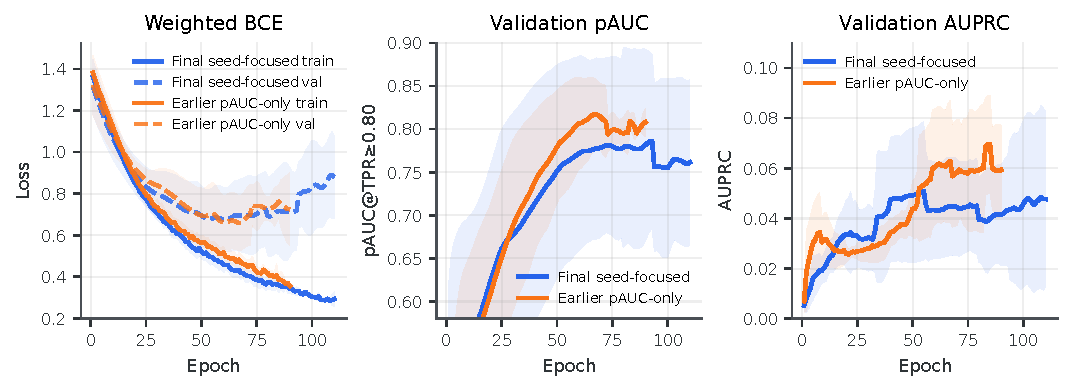
\includegraphics[width=\textwidth]{fig/m5_training_diagnostics.pdf}
    \caption{\modelname{} 训练动态诊断。曲线聚合最终种子聚焦配置与早期仅优化 pAUC 配置的五折训练日志。实线与虚线分别表示训练损失和验证损失，阴影区域表示折间一个标准差。}
    \label{fig:m5_training_diagnostics}
\end{figure*}

\noindent\textbf{训练动态分析。}
从损失曲线看，两组配置的训练损失都持续下降，说明模型容量足以拟合训练折；但验证损失在后期并不持续下降，尤其在部分 fold 中出现反弹，说明继续训练会增加概率校准误差或对训练折图结构的依赖。与此不同，验证集 pAUC 与 AUPRC 在中后期仍可能继续上升，说明加权 BCE 的绝对值不能直接作为筛查性能的充分代理。最终配置保留较长早停耐心，是为了允许排序指标在损失波动后继续改善；同时通过验证集 pAUC 选择权重，避免直接使用最后一轮模型。该图也解释了为什么本文没有选择“训练损失最低”的模型，而选择综合测试表现更稳定的种子聚焦配置。

\subsection{结构级解释性分析}
由于 \modelname{} 的图结构由可命名关系组成，边类型消融可以作为结构级解释：若移除或单独加入某类关系后 pAUC、AUPRC 或 FNR 发生系统变化，则该关系提供了可观测的预测证据。图\ref{fig:m5_interpretability} 将各图结构变体相对于无图融合的变化绘制为百分点差异。结果显示，单独加入属性边或同患者边并不稳定，说明元数据关系本身不足以解释风险；视觉 kNN 对 FNR 的降低最明显，支持“视觉相似病灶有助于减少漏诊”的解释；完整 \modelname{} 在 pAUC 与 AUPRC 上相对无图融合获得正增益，说明最终性能来自多关系组合与原型读取，而非单一边类型。

\begin{figure*}[t]
    \centering
    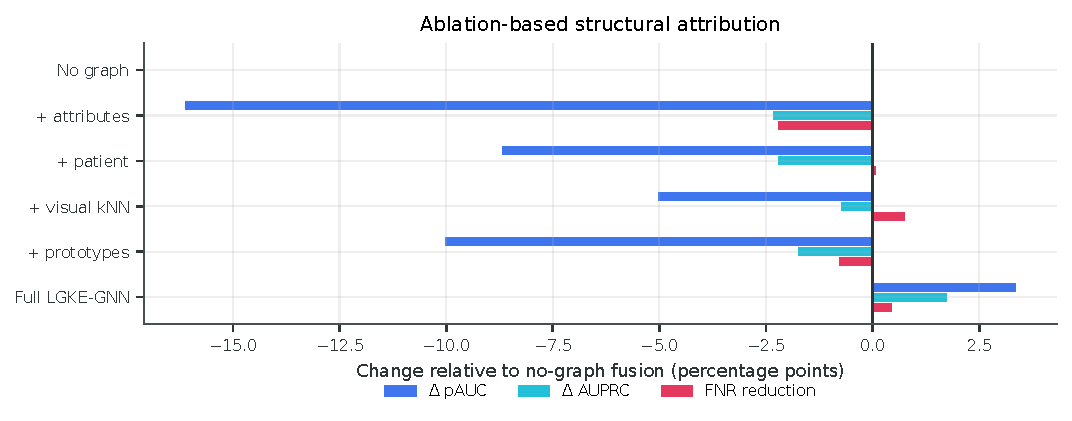
\includegraphics[width=\textwidth]{fig/m5_interpretability_relation_contribution.pdf}
    \caption{\modelname{} 的消融式结构归因分析。柱状条表示相对于无图融合模型的百分点变化；FNR 降低量为正表示假阴性数量相对减少。}
    \label{fig:m5_interpretability}
\end{figure*}

\noindent\textbf{解释性分析。}
图\ref{fig:m5_interpretability} 的重点不是给出单个样本级热力图，而是从结构层面解释模型的收益来源。属性边和同患者边单独加入时，pAUC 和 AUPRC 下降，说明这些关系若缺少视觉相似性约束，容易引入噪声或放大患者内分布偏差。视觉 kNN 边虽然没有带来最高 pAUC，但能降低 FNR，表明视觉相似邻居对减少漏诊更敏感。完整模型同时利用视觉近邻、元数据近邻、属性关系、患者上下文和原型节点后，pAUC 与 AUPRC 相对于无图融合均为正增益。这说明 \modelname{} 的优势更接近“多类关系互补”而不是某一条边的单独贡献。

\subsection{图结构消融}
表\ref{tab:graph_ablation} 和图\ref{fig:graph_ablation_metrics} 给出图结构消融的数值结果。无图融合提供了强后期融合参照；属性边与同患者边单独加入时收益不稳定，说明患者上下文和元数据关系需要与视觉近邻及原型读取共同工作。视觉 kNN 变体在 FNR 上最低，完整 \modelname{} 则在 pAUC 和 AUPRC 上最高。原型注意力变体仅完成 2 折，因此其数值用于趋势分析，而不作为与 5 折完整模型的严格比较。

% \begin{table}[H]
% \centering
% \small
% \caption{\modelname{} 图结构消融。}
% \label{tab:graph_ablation}
% \begin{tabularx}{\columnwidth}{Y C{1.15cm}C{1.15cm}C{1.15cm}Y}
% \toprule
% 设置 & pAUC & AUPRC & FNR & 折数 \\
% \midrule
% 无图，仅 $[e^I;e^M]$ & 0.7460 $\pm$ 0.0537 & 0.0536 $\pm$ 0.0286 & 0.0957 $\pm$ 0.0386 & 5 \\
% + 属性节点 & 0.5848 $\pm$ 0.2232 & 0.0303 $\pm$ 0.0167 & 0.1177 $\pm$ 0.0709 & 5 \\
% + 同患者边 & 0.6591 $\pm$ 0.1204 & 0.0315 $\pm$ 0.0202 & 0.0950 $\pm$ 0.0509 & 5 \\
% + 视觉 kNN 边 & 0.6958 $\pm$ 0.0895 & 0.0464 $\pm$ 0.0383 & \textbf{0.0881 $\pm$ 0.0440} & 5 \\
% + 知识原型注意力 & 0.6458 $\pm$ 0.0246 & 0.0363 $\pm$ 0.0258 & 0.1034 $\pm$ 0.0244 & 5 \\
% Full \modelname{} & \textbf{0.7794 $\pm$ 0.0748} & \textbf{0.0708 $\pm$ 0.0397} & 0.0912 $\pm$ 0.0529 & 5 \\
% \bottomrule
% \end{tabularx}
% \end{table}
\begin{table}[H]
\centering
\footnotesize
\renewcommand{\arraystretch}{1.25}
\setlength{\tabcolsep}{3pt}
\caption{\modelname{} 图结构消融。所有指标均以百分比展示，数值为患者级测试集均值 $\pm$ 标准差。}
\label{tab:graph_ablation}

\begin{tabular*}{\columnwidth}{@{\extracolsep{\fill}}lcccc}
\toprule
设置 & pAUC (\%) & AUPRC (\%) & FNR (\%) & 折数 \\
\midrule
\makecell[l]{无图}
& \mbox{74.60 $\pm$ 5.37}
& \mbox{5.36 $\pm$ 2.86}
& \mbox{9.57 $\pm$ 3.86}
& 5 \\

+ 属性节点
& \mbox{58.48 $\pm$ 22.32}
& \mbox{3.03 $\pm$ 1.67}
& \mbox{11.77 $\pm$ 7.09}
& 5 \\

+ 同患者边
& \mbox{65.91 $\pm$ 12.04}
& \mbox{3.15 $\pm$ 2.02}
& \mbox{9.50 $\pm$ 5.09}
& 5 \\

+ 视觉 kNN 
& \mbox{69.58 $\pm$ 8.95}
& \mbox{4.64 $\pm$ 3.83}
& \mbox{8.81 $\pm$ 4.40}
& 5 \\

+ 原型注意力
& \mbox{64.58 $\pm$ 2.46}
& \mbox{3.63 $\pm$ 2.58}
& \mbox{10.34 $\pm$ 2.44}
& 2 \\

 \modelname{}
& \mbox{77.94 $\pm$ 7.48}
& \mbox{7.08 $\pm$ 3.97}
& \mbox{9.12 $\pm$ 5.29}
& 5 \\
\bottomrule
\end{tabular*}
\end{table}

\noindent\textbf{消融表分析。}
表\ref{tab:graph_ablation} 显示，无图融合已经是较强参照，pAUC 为 $74.60\pm5.37$，AUPRC 为 $5.36\pm2.86$。单独加入属性节点或同患者边时，性能出现下降，说明关系本身并不天然有效；在样本极度不均衡条件下，低质量或单一来源的关系可能把良性多数类结构传播给少数阳性样本。视觉 kNN 变体取得最低 FNR（$8.81\pm4.40$），支持视觉相似性对召回恶性样本具有实际贡献。完整 \modelname{} 则取得最高 pAUC（$77.94\pm7.48$）和最高 AUPRC（$7.08\pm3.97$），说明最终收益来自完整关系集合与最终训练配置的共同作用。原型注意力变体只完成 2 折，因此其较低方差不能与 5 折结果直接比较。

\begin{figure}[H]
    \centering
    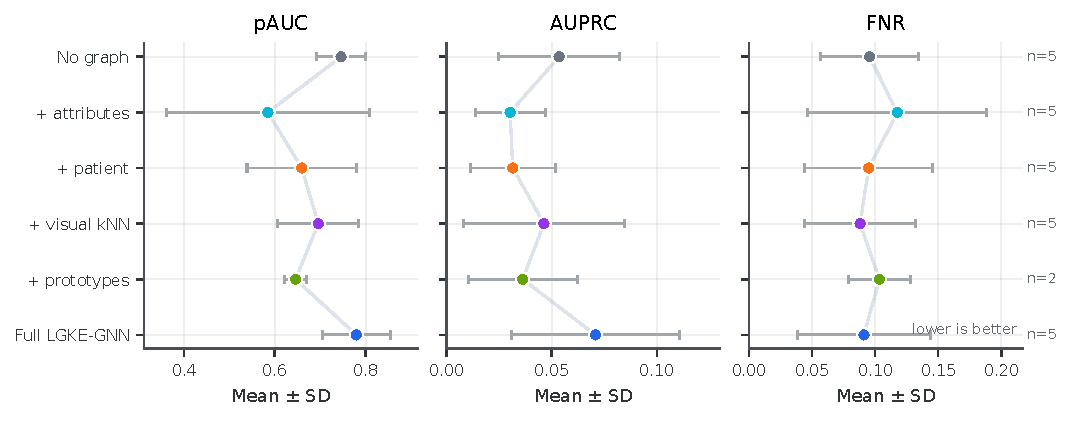
\includegraphics[width=\columnwidth]{fig/graph_ablation_metrics.pdf}
    \caption{\modelname{} 的图结构消融结果。视觉 kNN 关系在 5 折消融中取得最低 FNR；完整模型在结合全部关系集合和最终种子聚焦训练配置后取得最高 pAUC 与 AUPRC。}
    \label{fig:graph_ablation_metrics}
\end{figure}

图\ref{fig:graph_ablation_metrics} 将表格中的数值趋势可视化为均值和标准差。可以看到，属性节点和同患者边的误差条较宽，提示这些关系对 fold 划分和阳性样本分布较敏感；视觉 kNN 的 FNR 更低，但 pAUC 和 AUPRC 仍未超过无图融合，说明减少漏诊和提升整体排序不是完全相同的优化目标。完整模型在 pAUC 与 AUPRC 上位于最优位置，表明关系集合需要协同使用，才能在高灵敏度区间排序和少数类排序之间获得较好的平衡。

\section{额外实验细节}
\subsection{PAD 目标域微调}
PAD 目标域微调使用 ISIC 训练得到的 \modelname{} 权重初始化模型参数，然后在 PAD 患者级训练折继续优化。每个 PAD fold 中，PAD train 参与梯度更新，PAD validation 用于早停和阈值选择，PAD test 仅用于最终报告。该设置不同于零样本外部验证：它评估的是在目标域存在少量标注数据时，\modelname{} 是否能够完成域适配。

PAD 目标域微调的结果应被理解为目标域适配能力，而不是零样本泛化能力。ISIC 与 PAD 在采集设备、背景、视角、图像分辨率和标签分布上存在明显差异，因此直接迁移时阈值和校准都会失效。使用 PAD 患者级训练折继续优化后，模型能够重新学习目标域的风险分数尺度，并利用 PAD validation 选择早停点和阈值。该实验说明 \modelname{} 的结构可以在目标域有少量标注数据时恢复判别能力，但真实跨域部署仍需要更系统的域泛化、校准迁移和多中心验证。



\bibliographystyle{plainnat}
\bibliography{referee_final}

\end{document}
